\RequirePackage[l2tabu, orthodox]{nag}

\documentclass[10pt]{scrartcl}
% \documentclass[10pt]{article}
\usepackage[T1]{fontenc}
\usepackage{amsmath,amsfonts,amssymb}
\usepackage{mathtools}
\usepackage{color,soul}
\usepackage[margin=2cm]{geometry}
\usepackage{enumerate}
\usepackage{graphicx}
\usepackage[colorlinks=true,urlcolor=blue]{hyperref}
\usepackage{floatrow}
\usepackage{deluxetable}
\usepackage{verbatim}
\usepackage{fancyvrb}
\usepackage{listings}
\usepackage{calc}
\usepackage[font=small]{caption}
\usepackage[font=scriptsize]{subcaption}
\usepackage[activate={true,nocompatibility},final,tracking=true,kerning=true,spacing=true,factor=1100,stretch=10,shrink=10]{microtype}
\SetTracking{encoding={*}, shape=sc}{40}

\floatsetup{ 
  heightadjust=object,
  valign=t
}

\definecolor{Light}{gray}{.90}
\sethlcolor{Light}

\title{Pics of slats}
\author{Jeren Suzuki}
\date{Last Edited \today}

\begin{document}

\maketitle
\pagenumbering{Roman}
\tableofcontents
\clearpage
\pagenumbering{arabic}

\section{Introduction} % (fold)
\label{sec:introduction}
Just some pictures of slats taken on Friday, August 2, 2013. Testing out how pictures look according to lighting conditions and setup. The photos were taken on a light table with a cardboard box on top. The box had a small cut out at the top to make room for the camera. Stencils of positions were drawn for a repeatable orientation.
% section introduction (end)

\section{Front light, without diffuse paper} % (fold)
\label{sec:front_light_with_diffuse_paper}
The worst of the configuraions, front lighting offered the least contrast between the background and slats. While arguably the most accurate color representation, who cares about that. 

\begin{figure}[!ht]
    \centering
    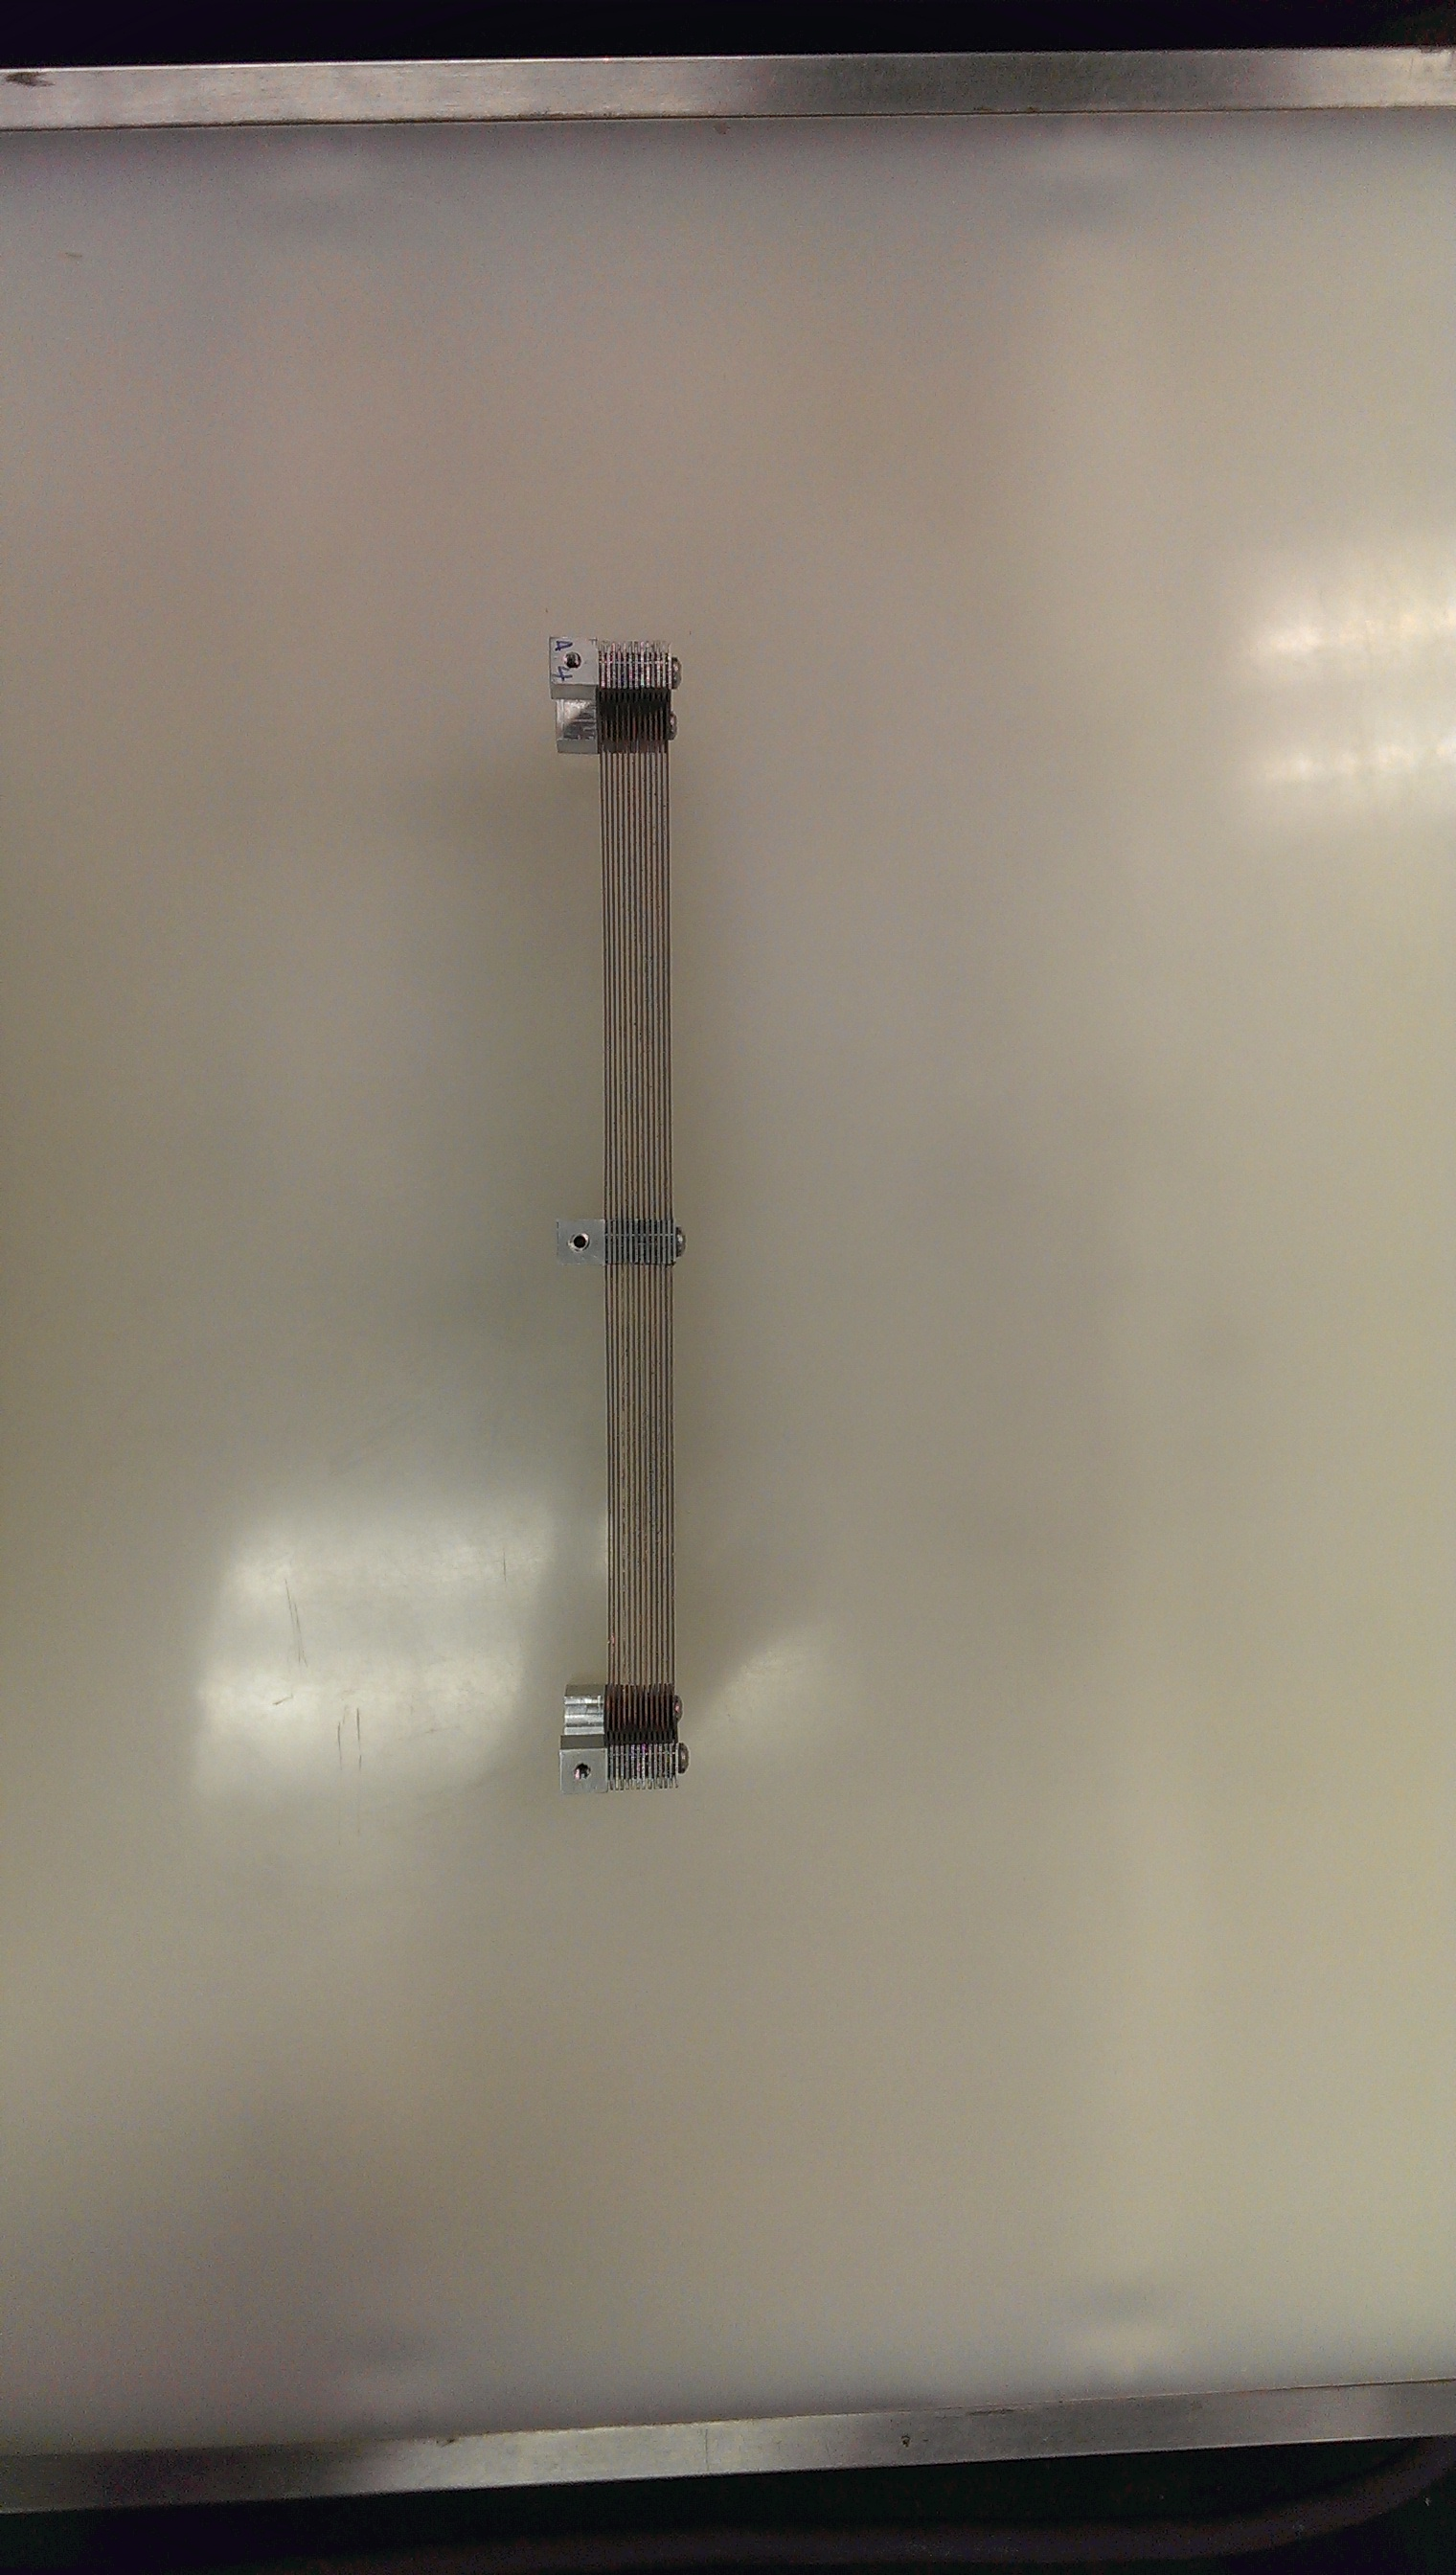
\includegraphics[width=.7\textwidth]{../plots_tables_images/slats/IMAG0151.jpg}    
    \caption{Front light, without diffuse paper}
\end{figure}

\begin{figure}[!ht]
    \centering
    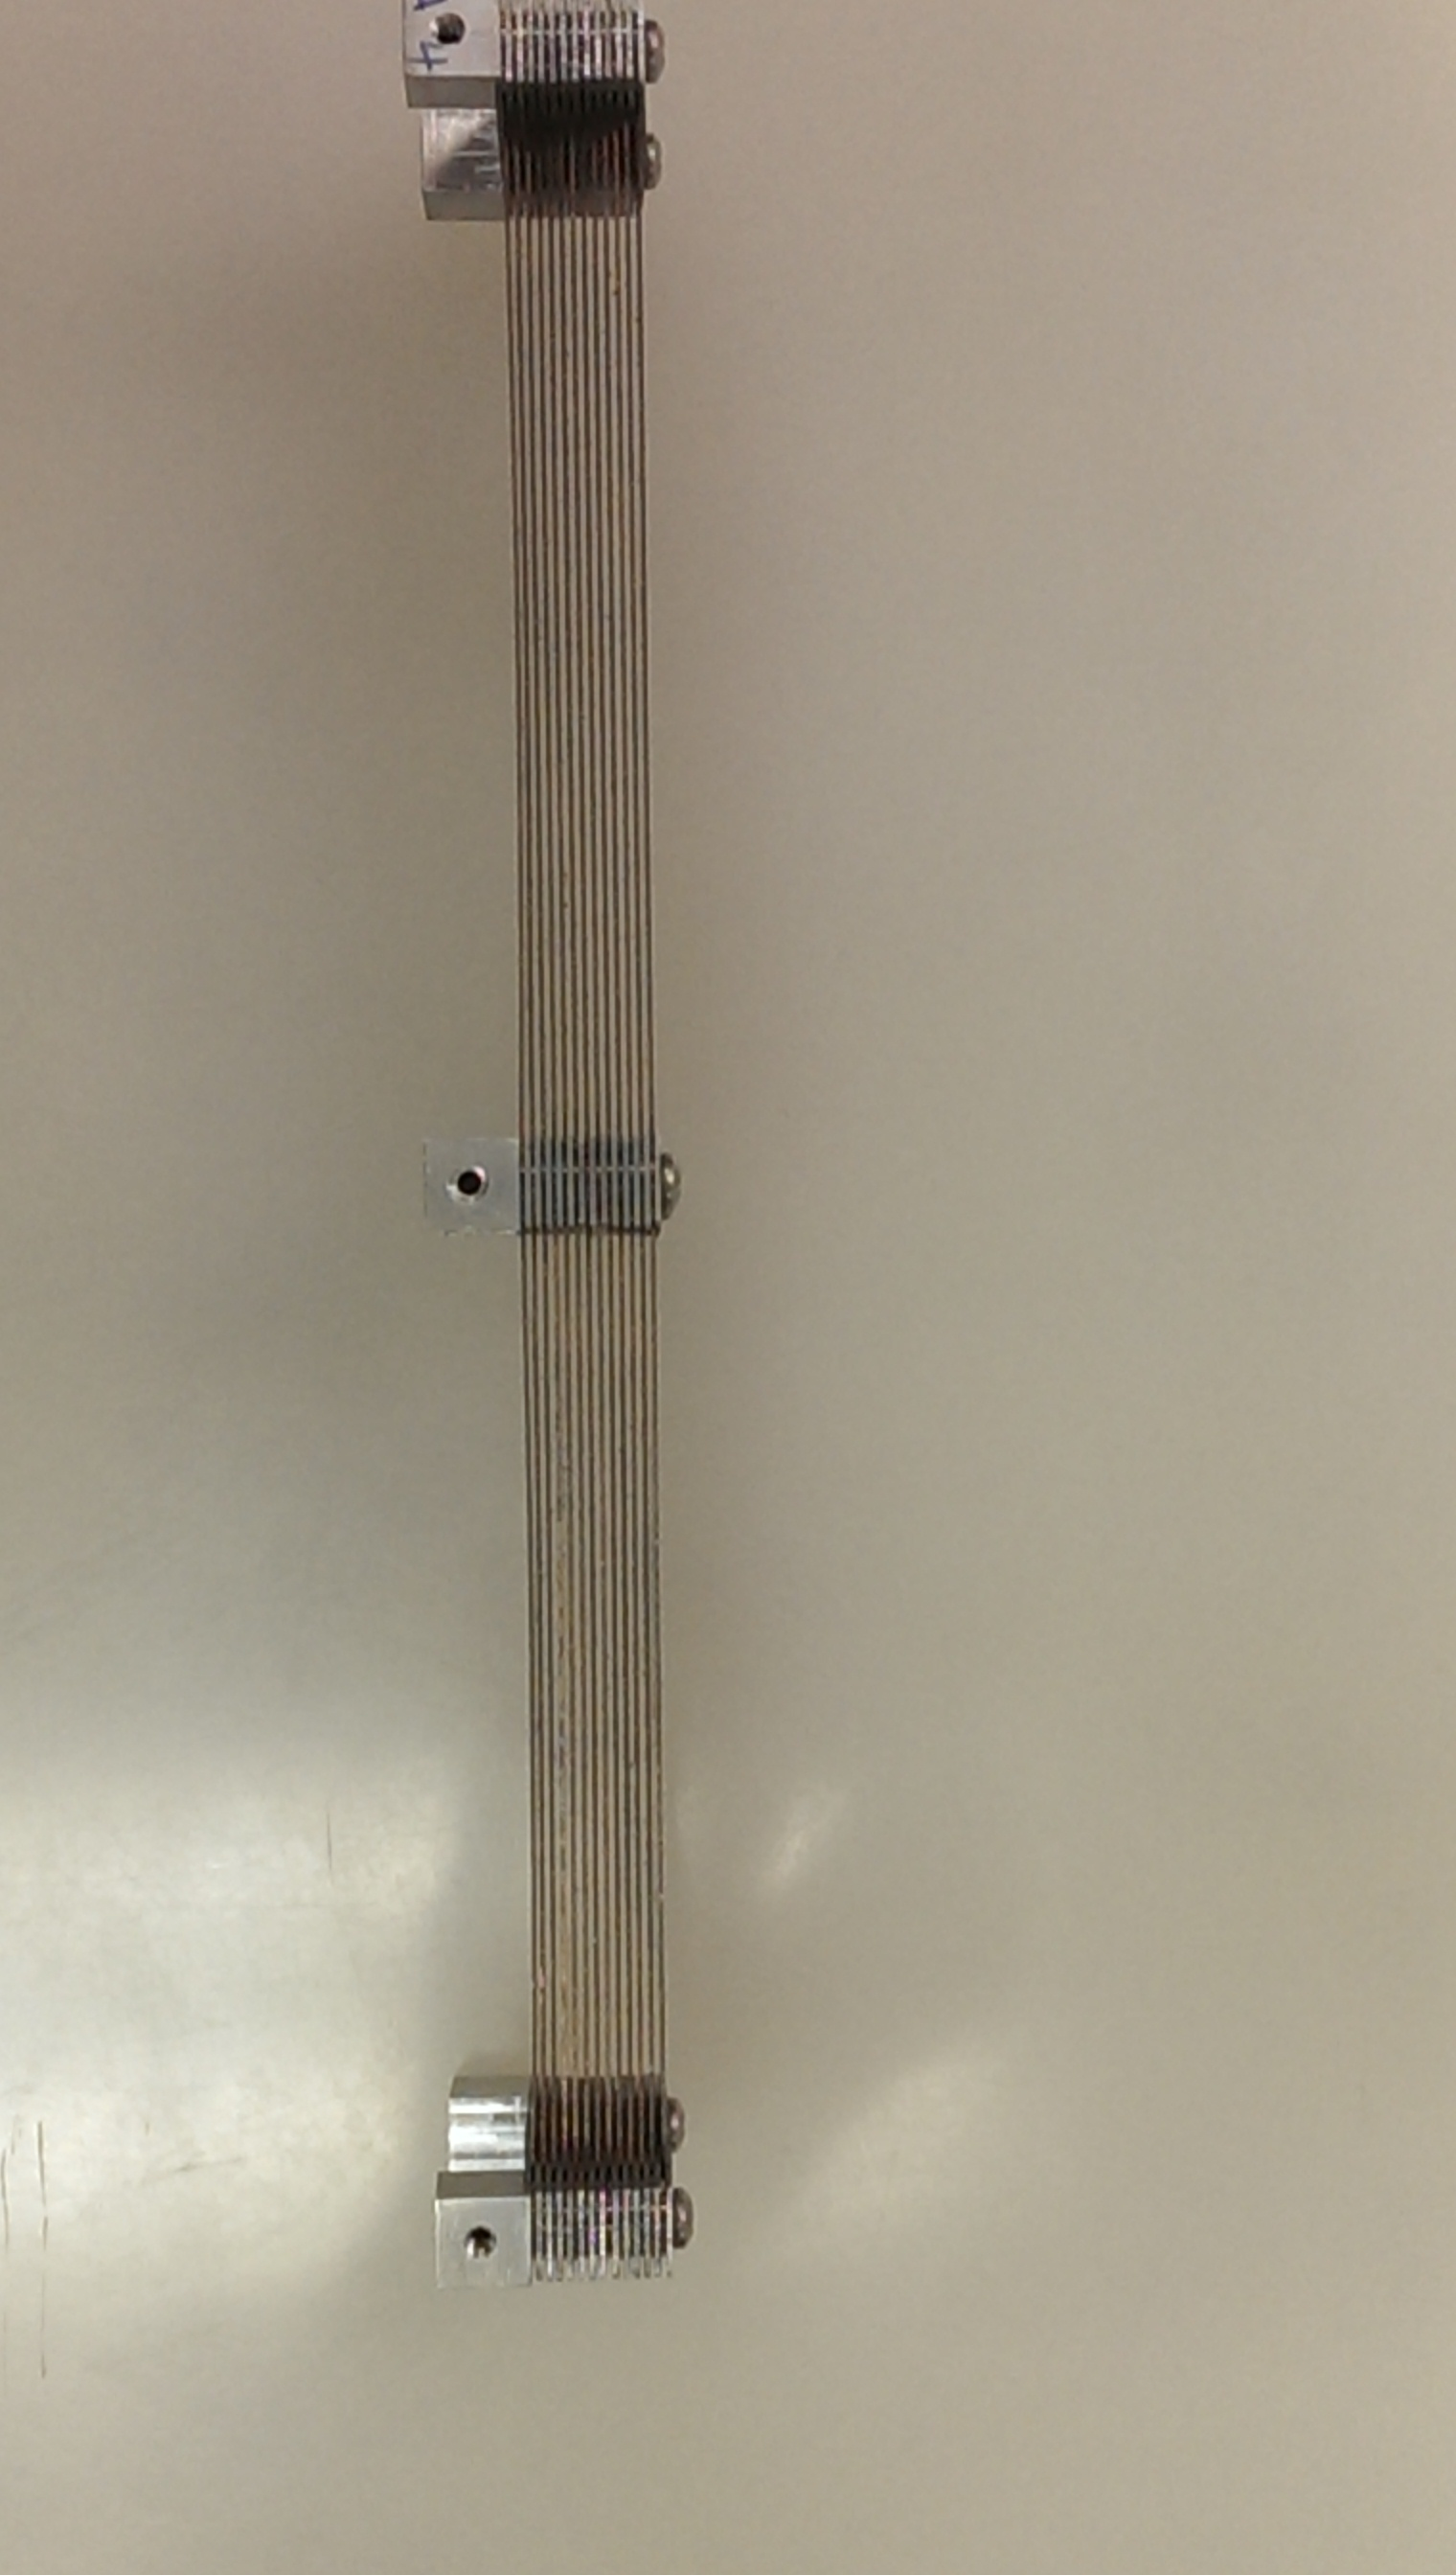
\includegraphics[width=.7\textwidth]{../plots_tables_images/slats/IMAG0150.jpg}    
    \caption{Zoomed in with camera phone so bundle would utilize more image space. Doesn't result in a better quality photo, just upscaled.}
\end{figure}
% section front_light_with_diffuse_paper (end)

\clearpage
\section{Back light, with diffuse paper} % (fold)
\label{sec:with_diffuse_paper}
We thought it a good idea to use some tissue paper to make the light more diffuse; it didn't provide any benefit. In fact, it added unwanted noise and dark splotches in the image. 

\begin{figure}[!ht]
    \ffigbox[][\FBheight]{%
    \begin{subfloatrow}[2]%
        \ffigbox[\FBwidth]%
       {%
       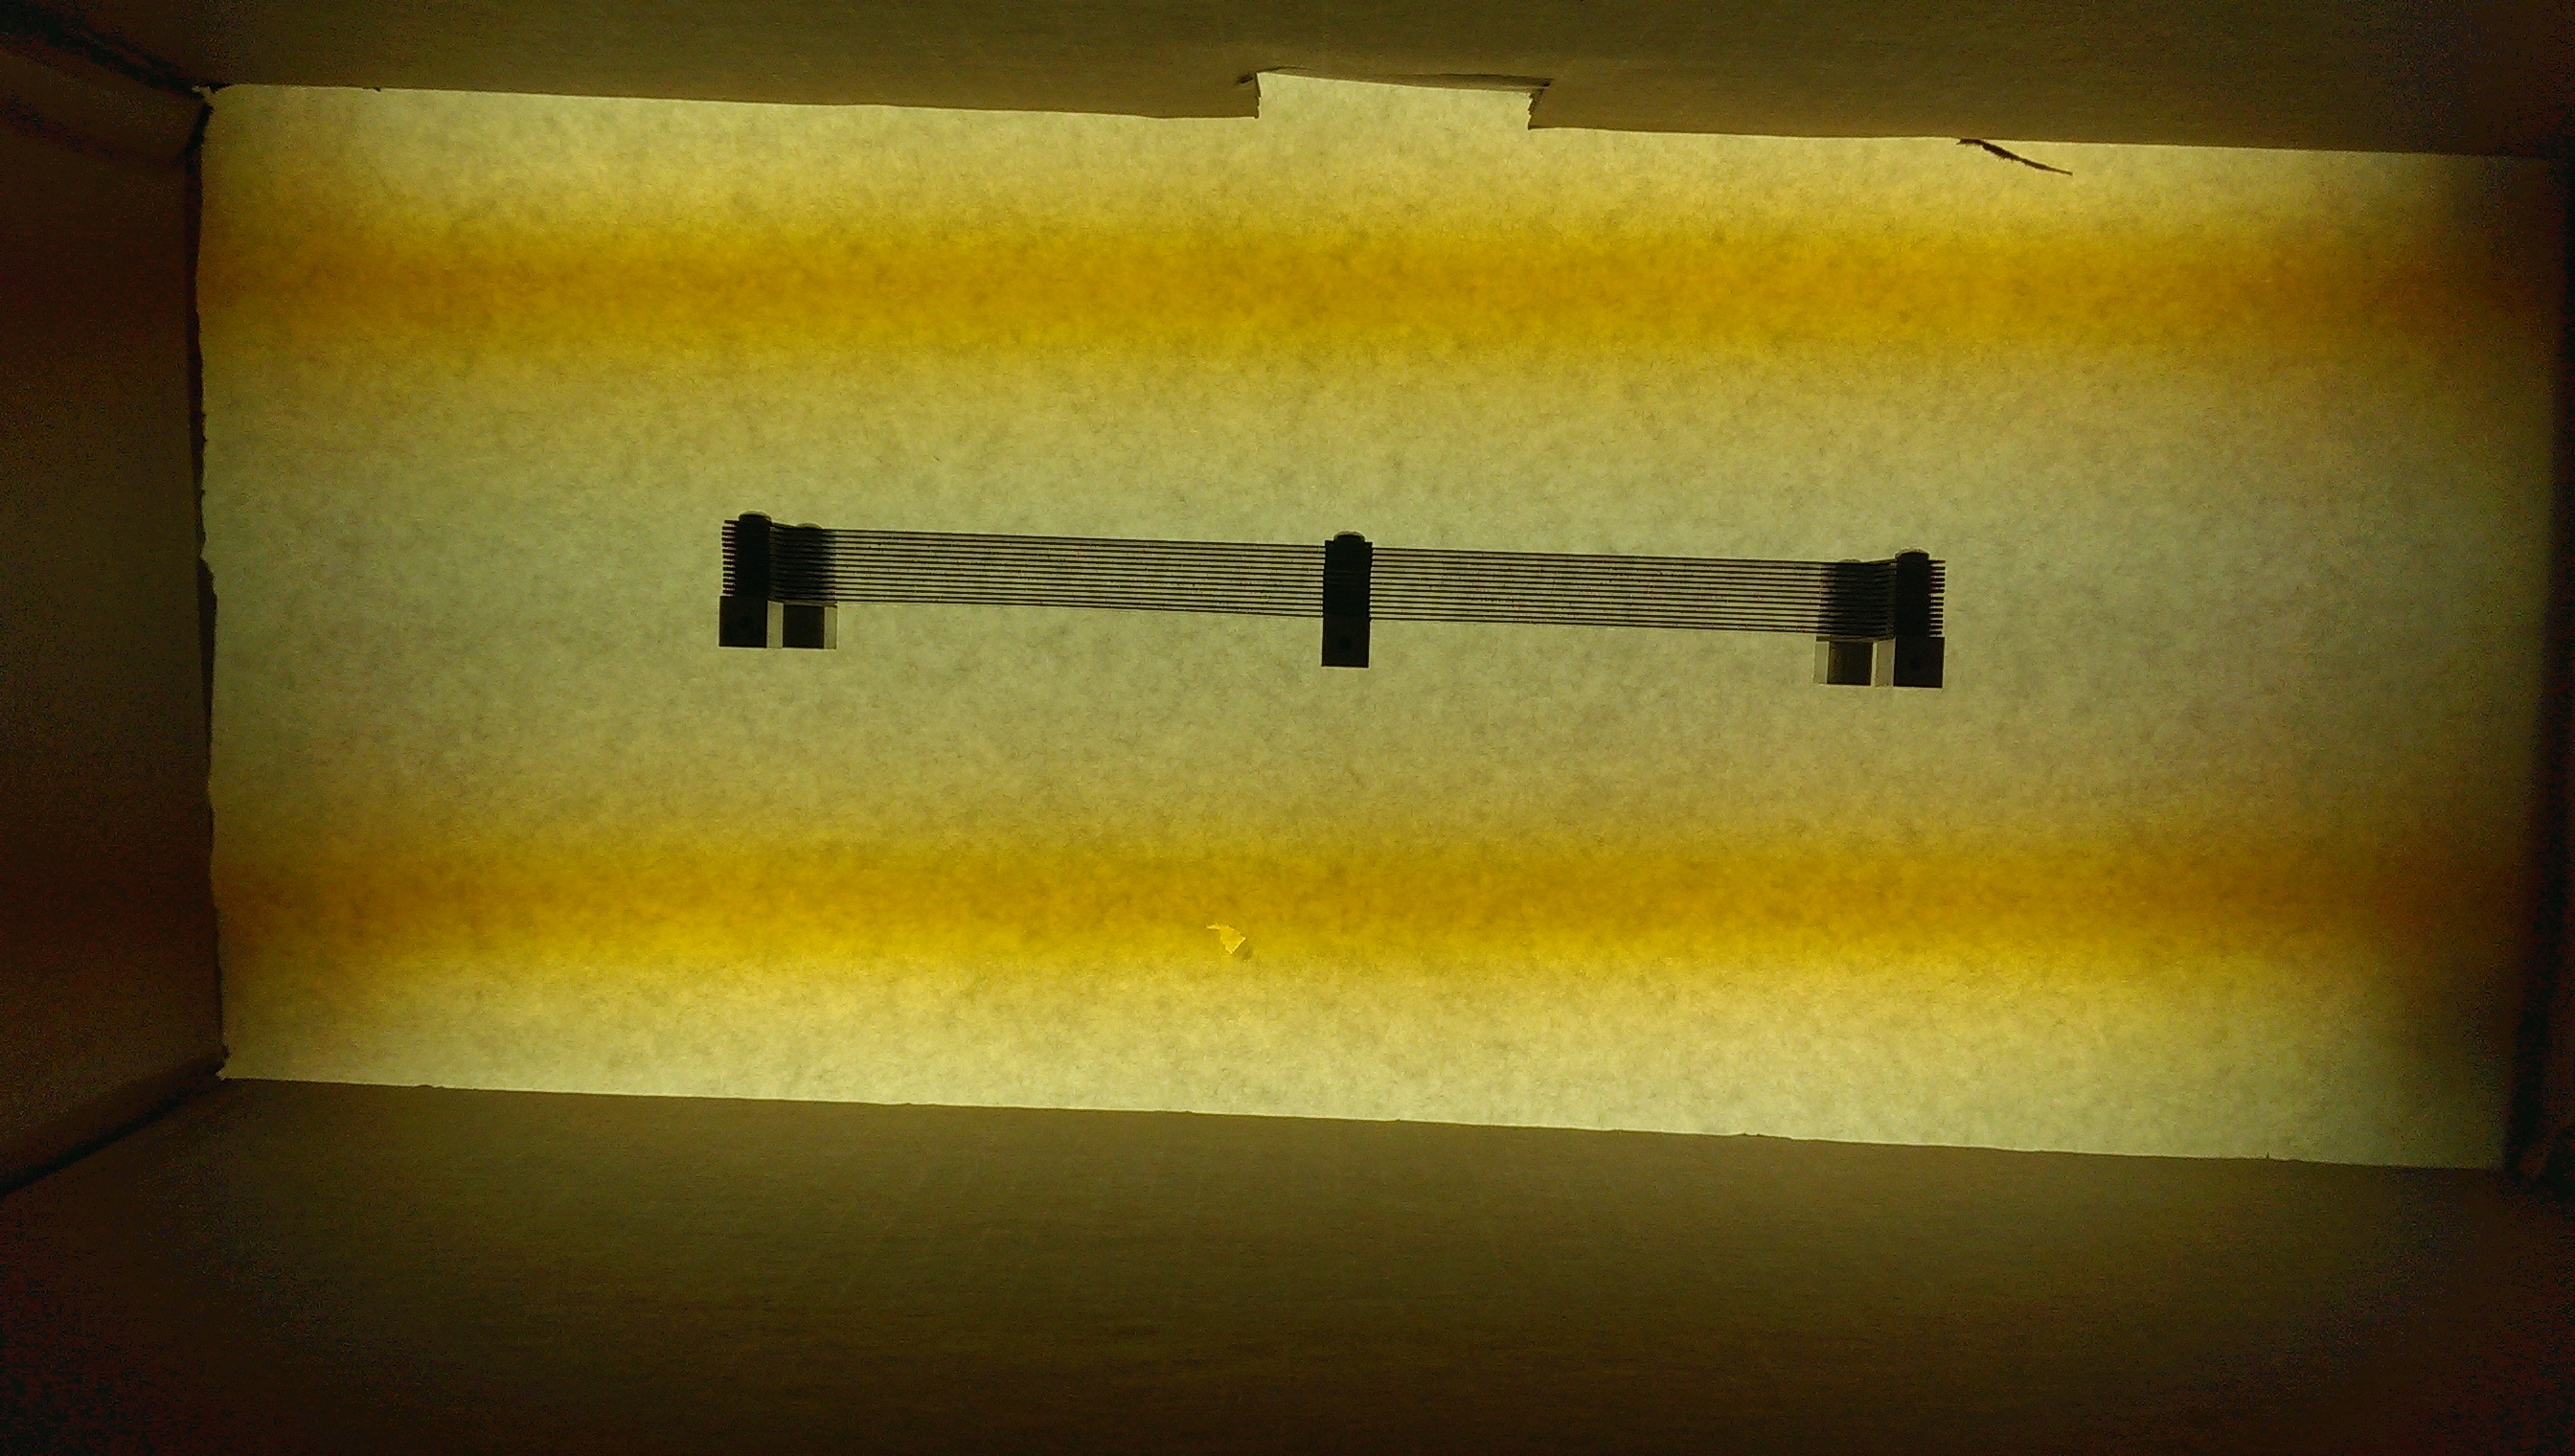
\includegraphics[width=.5\textwidth]{../plots_tables_images/slats/IMAG0116.jpg}%
       }%
       {%
       \caption{}%
       }%
        \ffigbox[\Xhsize]%
       {%
       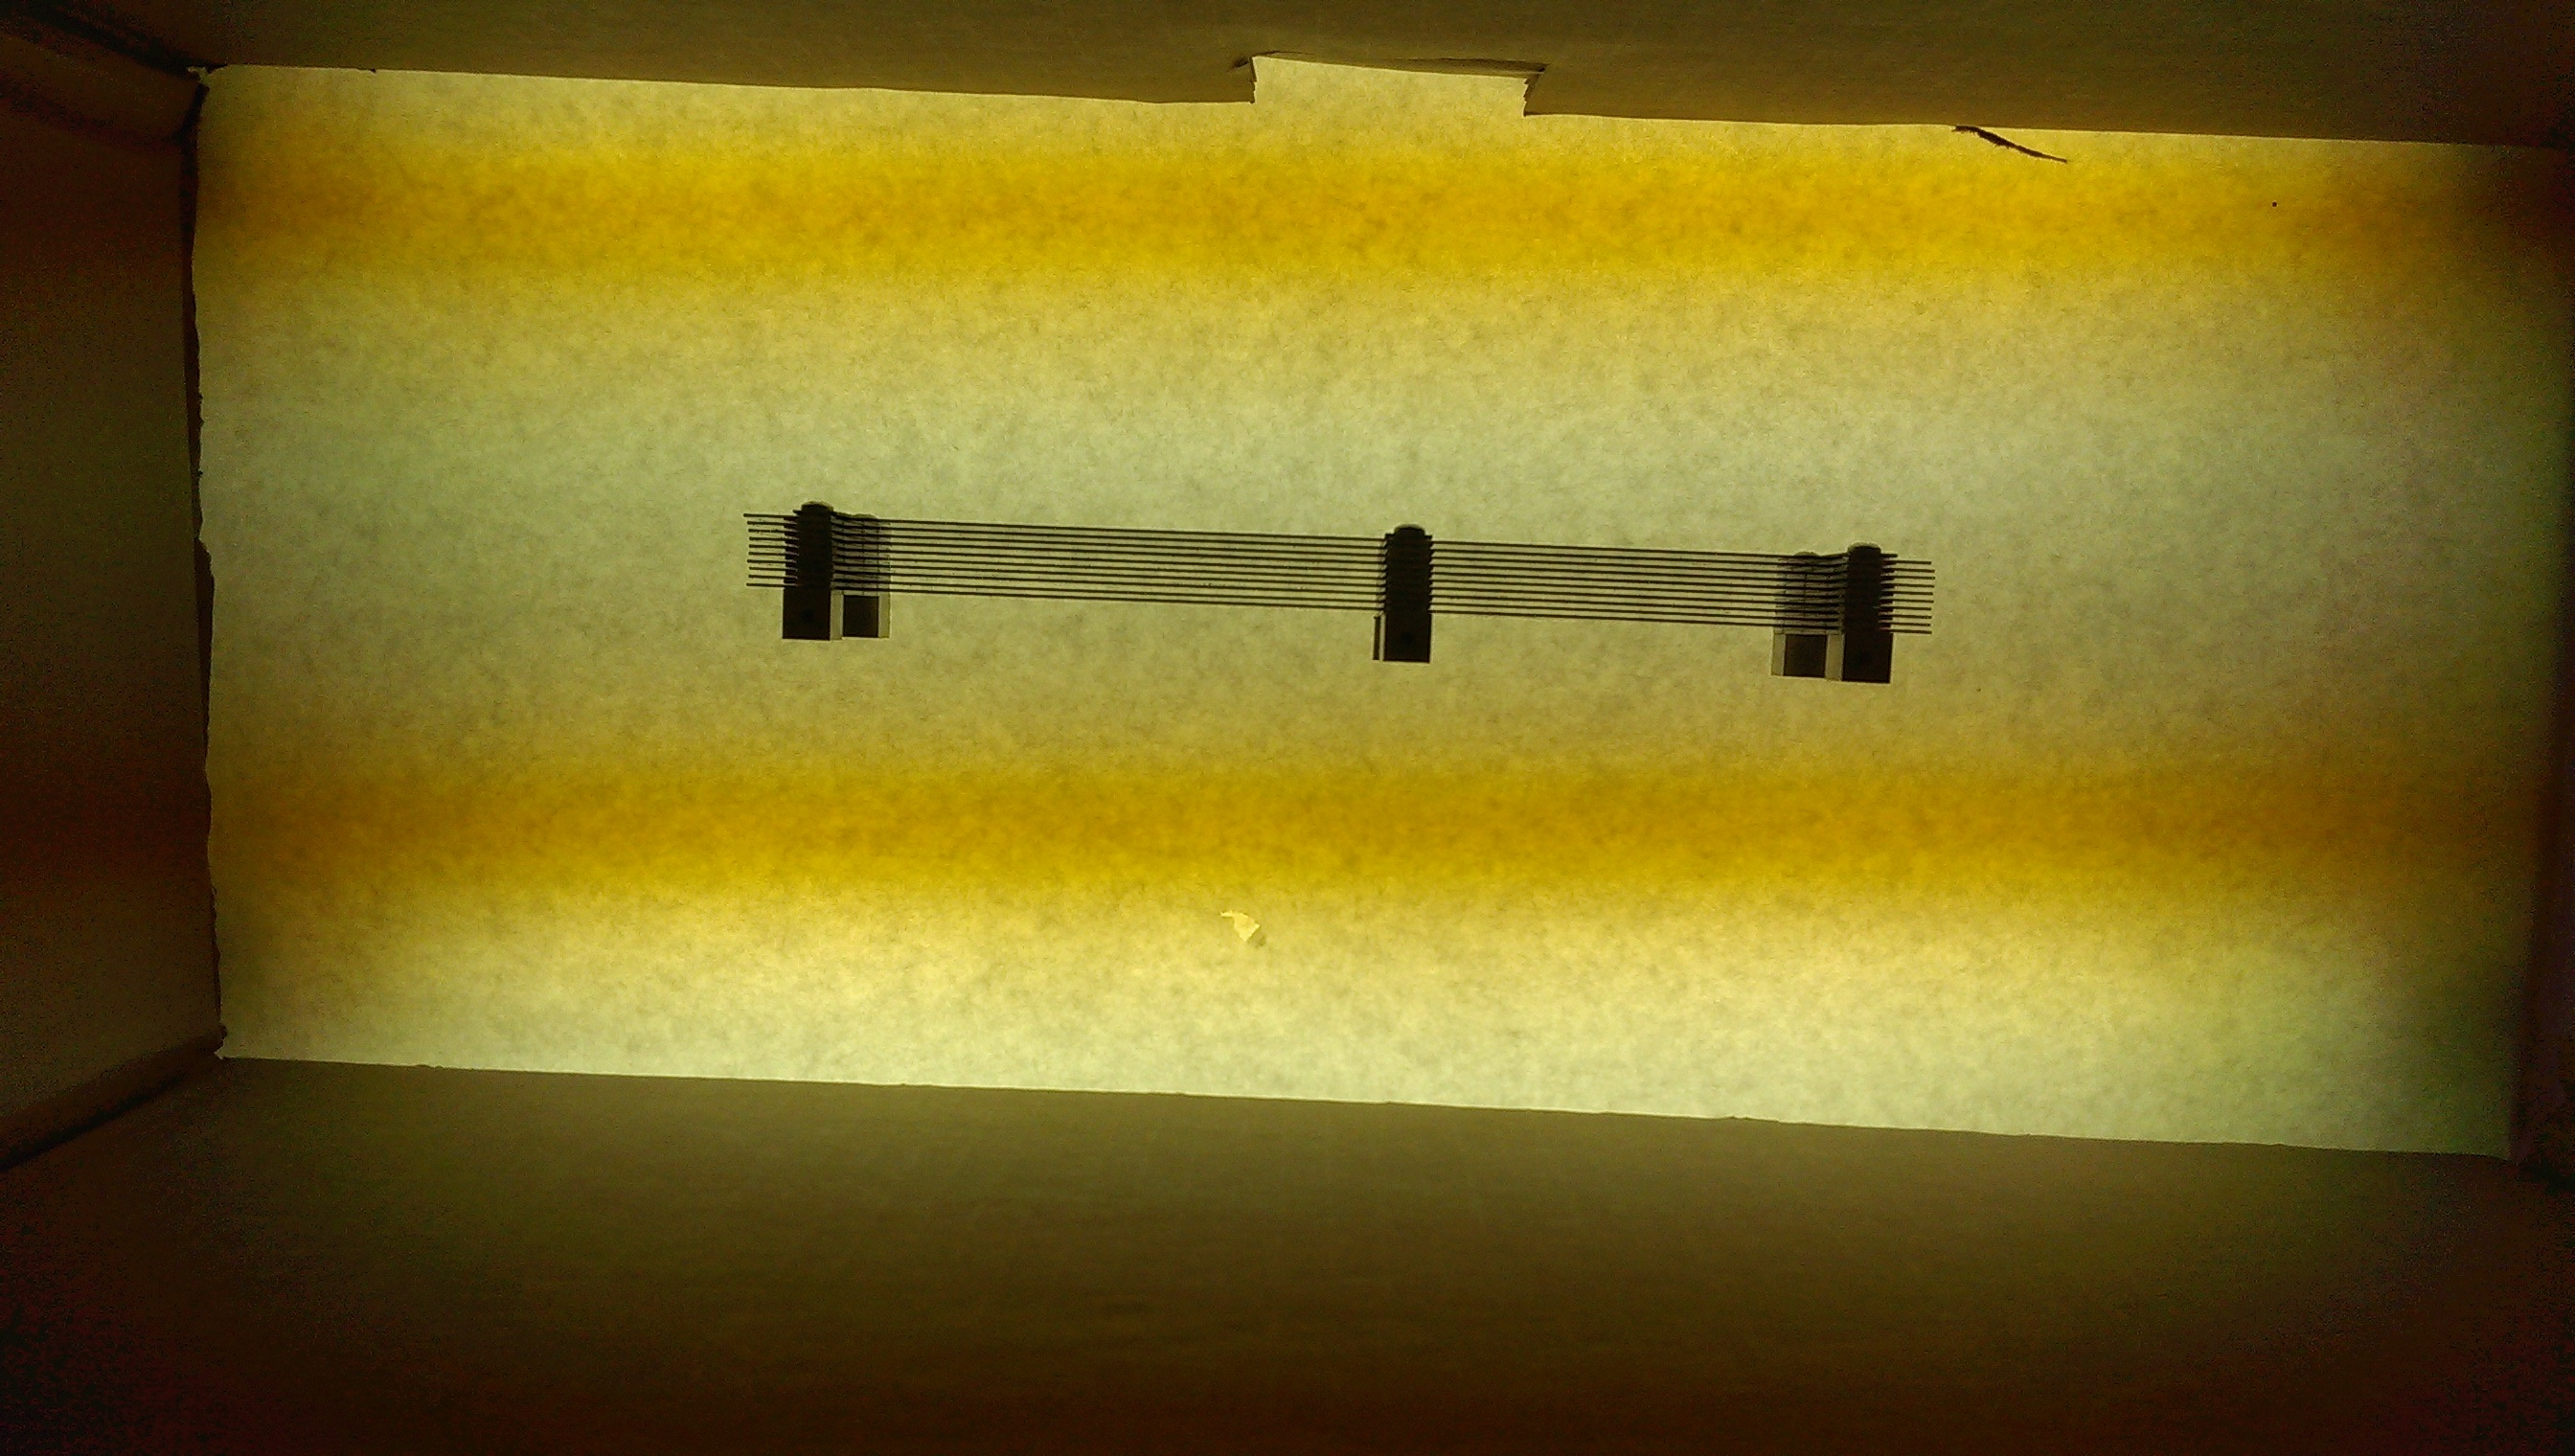
\includegraphics[width=.5\textwidth]{../plots_tables_images/slats/IMAG0120.jpg}%
       }%
       {%
       \caption{}%
       }%
    \end{subfloatrow}}

        \ffigbox[][\FBheight]{%
    \begin{subfloatrow}[2]%
        \ffigbox[\FBwidth]%
       {%
       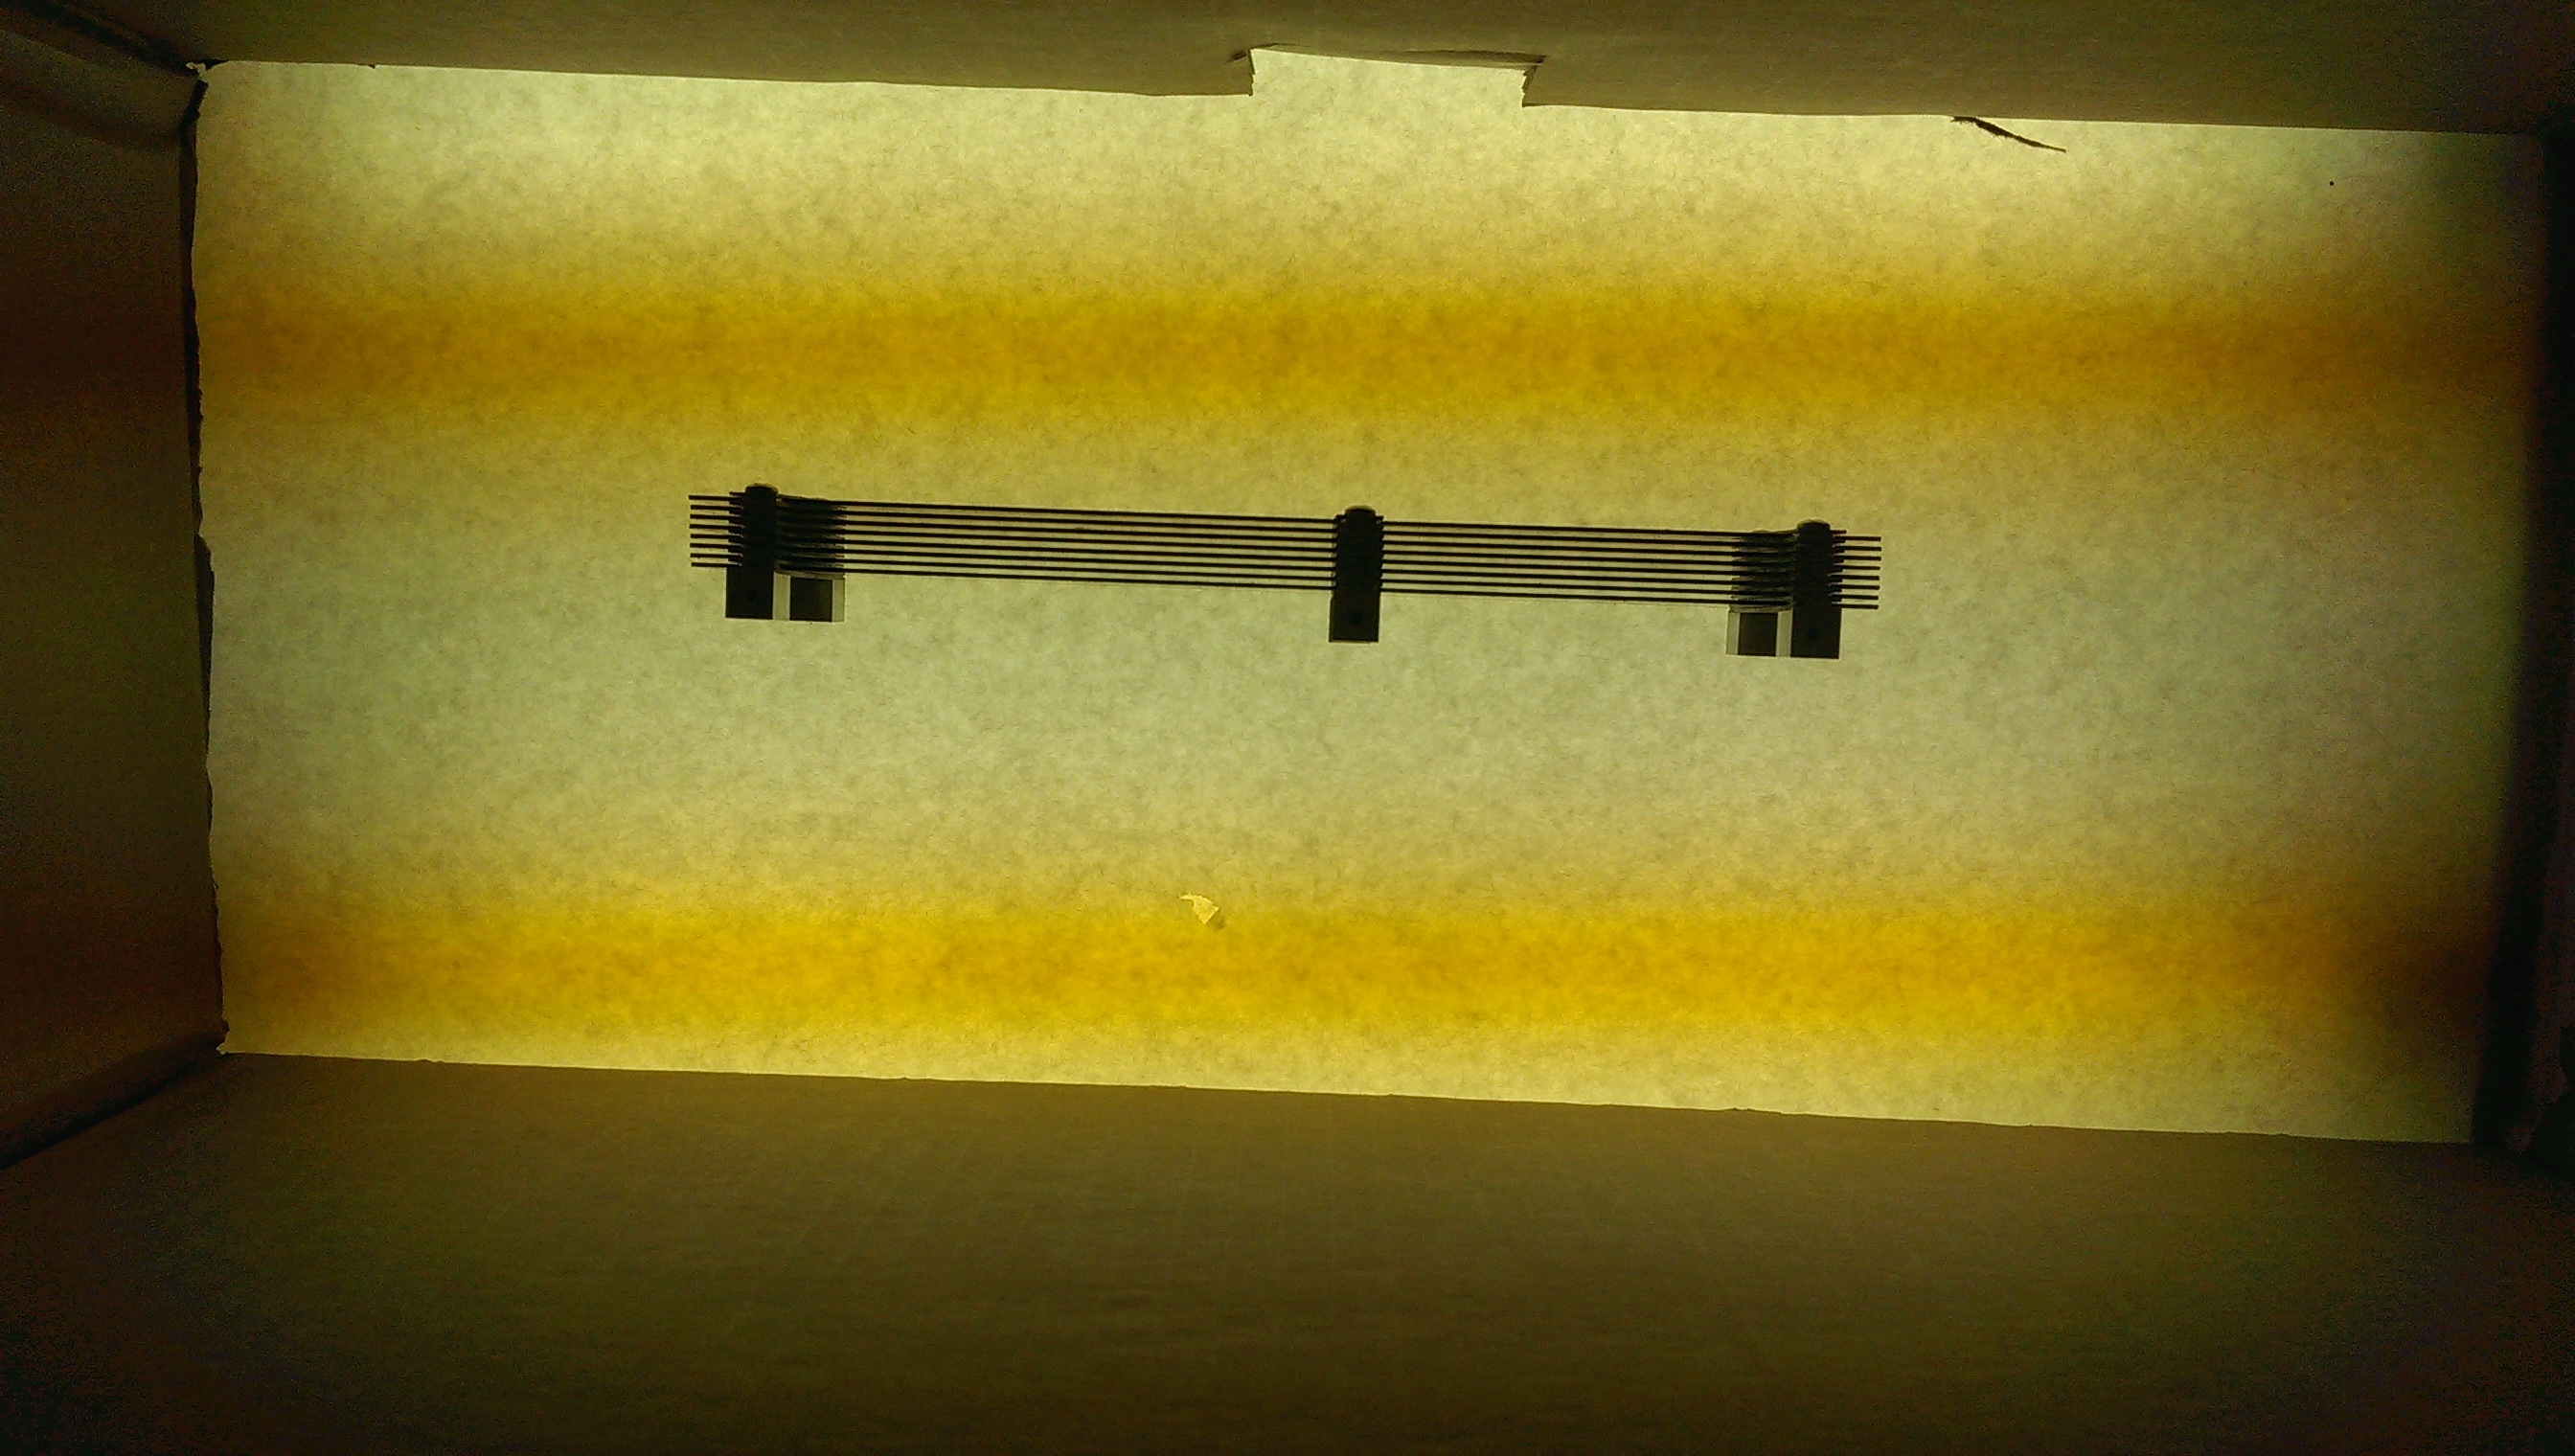
\includegraphics[width=.5\textwidth]{../plots_tables_images/slats/IMAG0124_BURST002_COVER.jpg}%
       }%
       {%
       \caption{}%
       }%
        \ffigbox[\Xhsize]%
       {%
       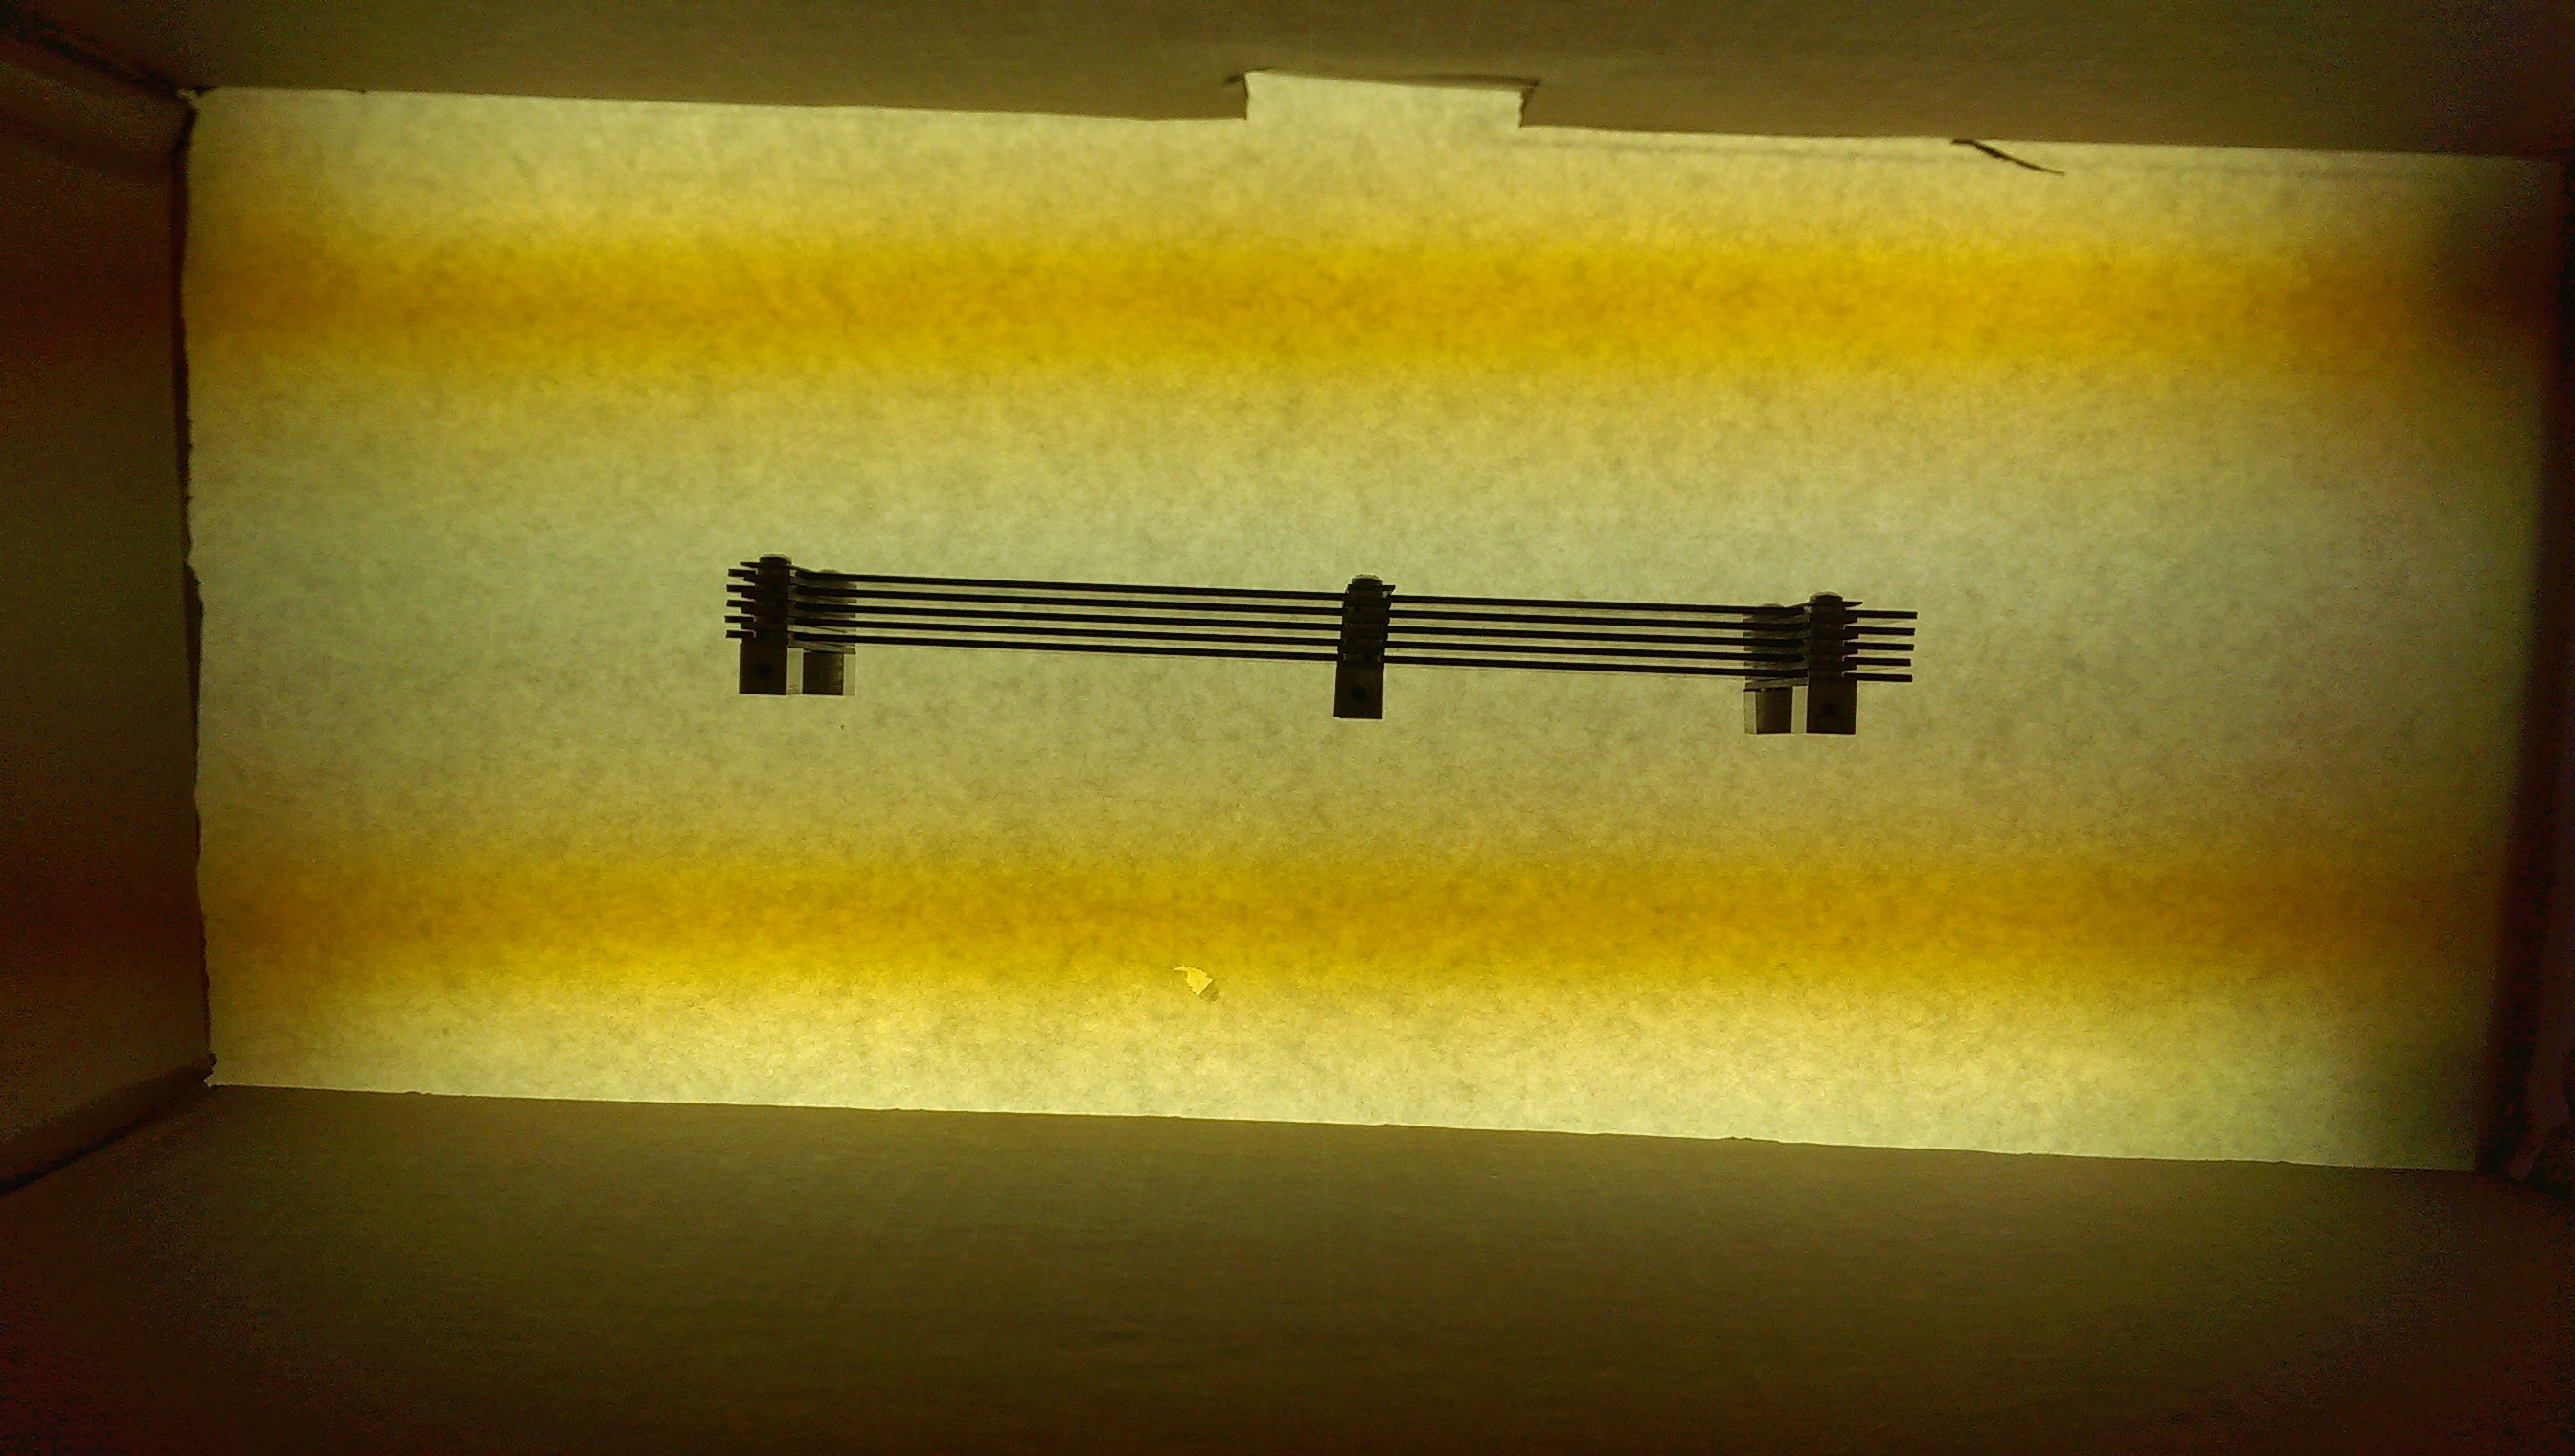
\includegraphics[width=.5\textwidth]{../plots_tables_images/slats/IMAG0133_BURST003.jpg}%
       }%
       {%
       \caption{}%
       }%
    \end{subfloatrow}}
    {\caption{Even though the images are small you can still zoom in a lot.}}%
\end{figure}

% \begin{figure}[!ht]
%     \centering
%     \hspace{-1.0in}
%     \begin{subfigure}[b]{.45\linewidth}
%         \centering
%         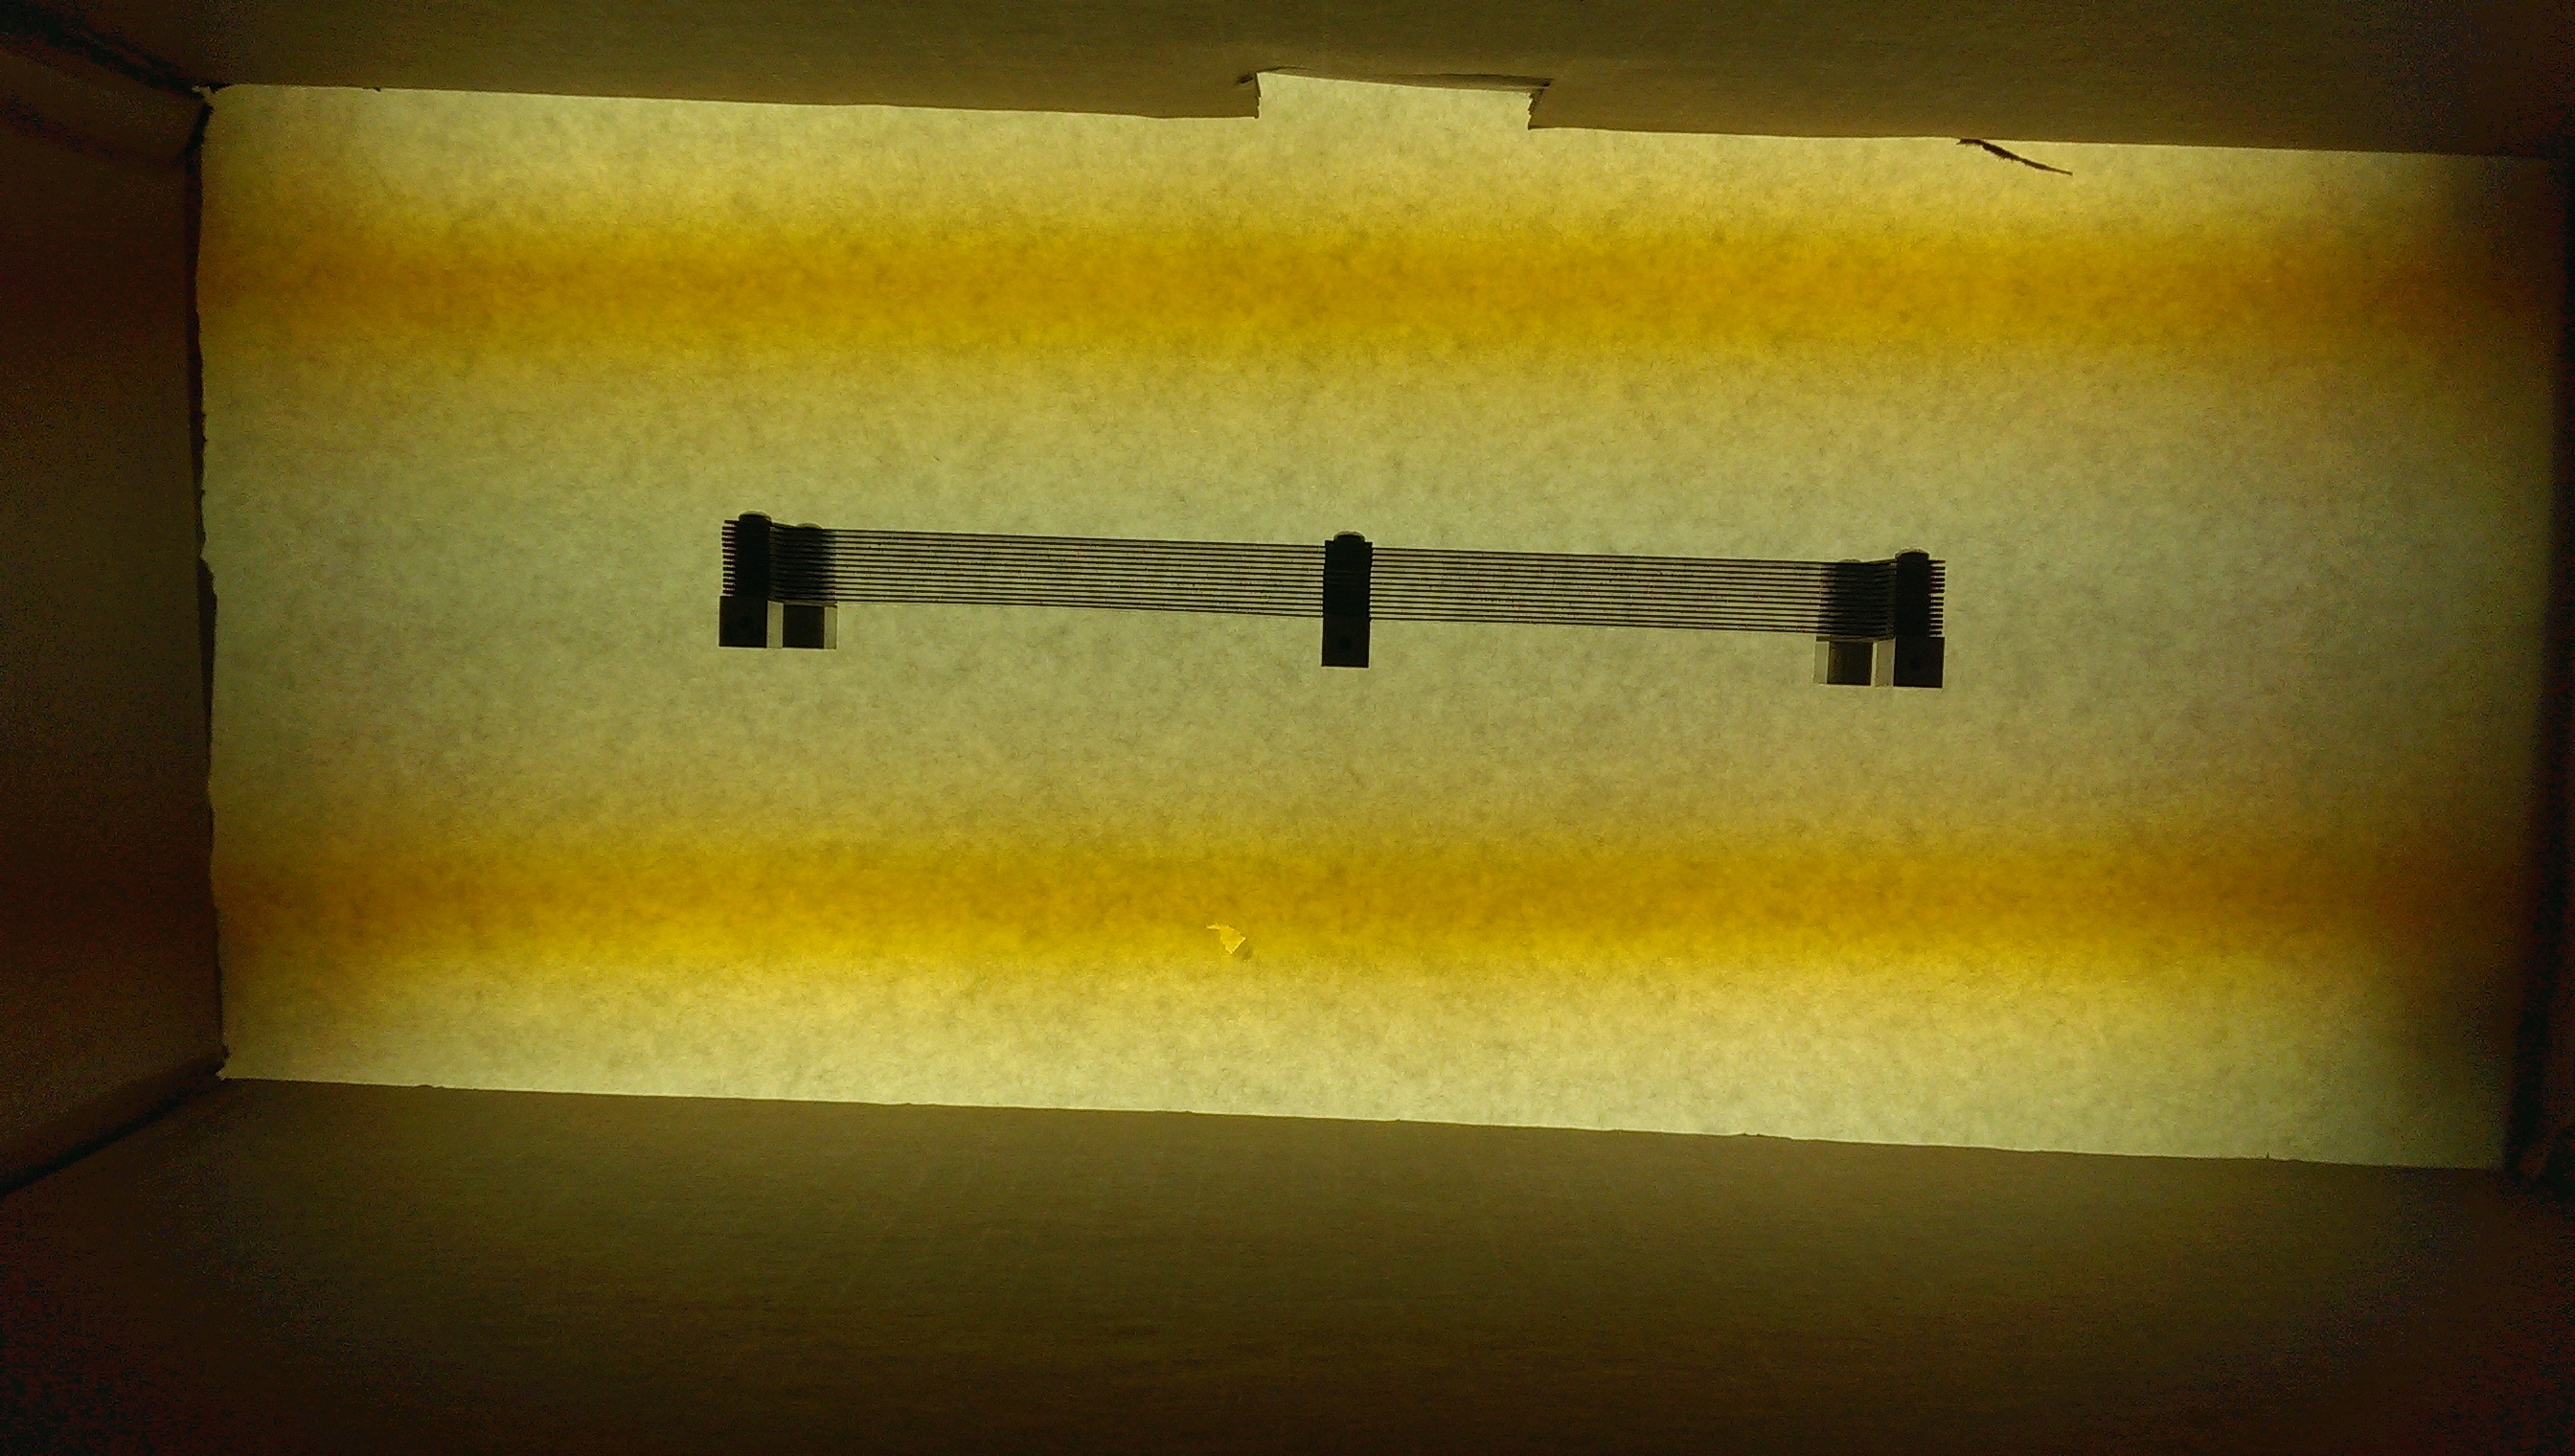
\includegraphics[width=1.3\textwidth]{../plots_tables_images/slats/IMAG0116.jpg}
%         \caption{}
%     \end{subfigure}
%     \hspace{.5in}
%     \begin{subfigure}[b]{.45\linewidth}
%         \centering
%         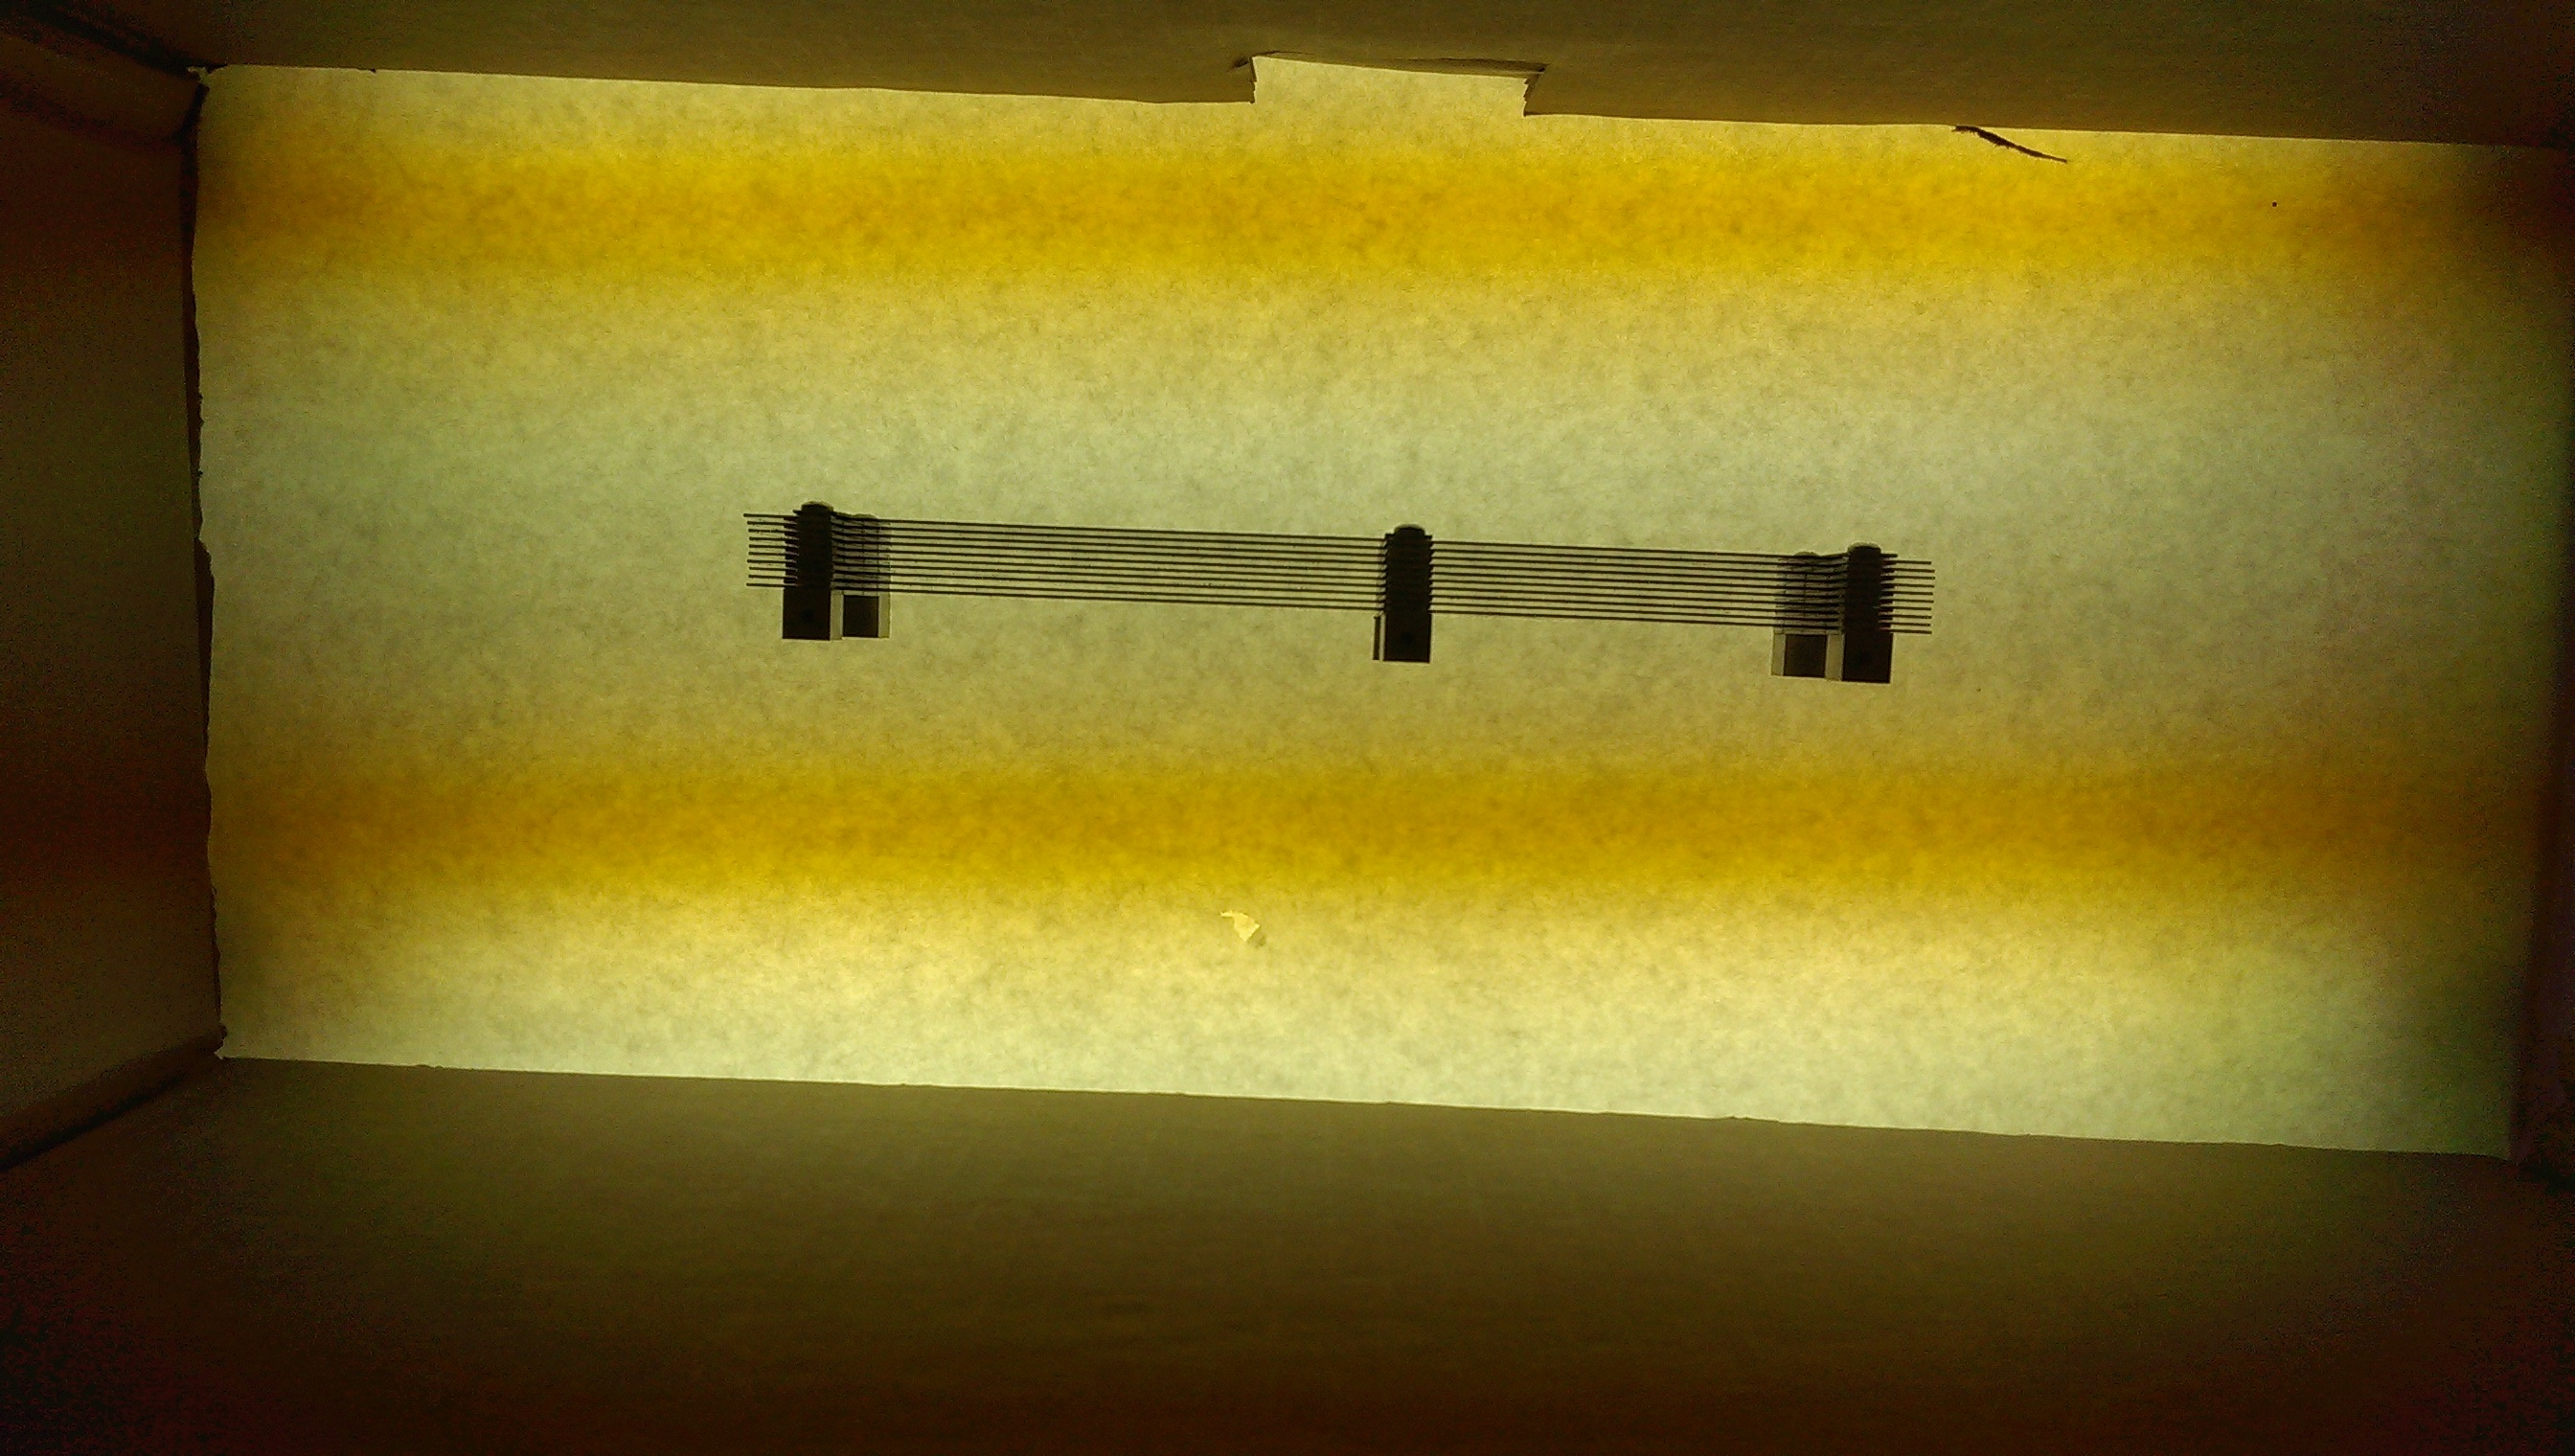
\includegraphics[width=1.3\textwidth]{../plots_tables_images/slats/IMAG0120.jpg}
%         \caption{}
%     \end{subfigure}

%     \hspace{-1.0in}
%     \begin{subfigure}[b]{.45\linewidth}
%         \centering
%         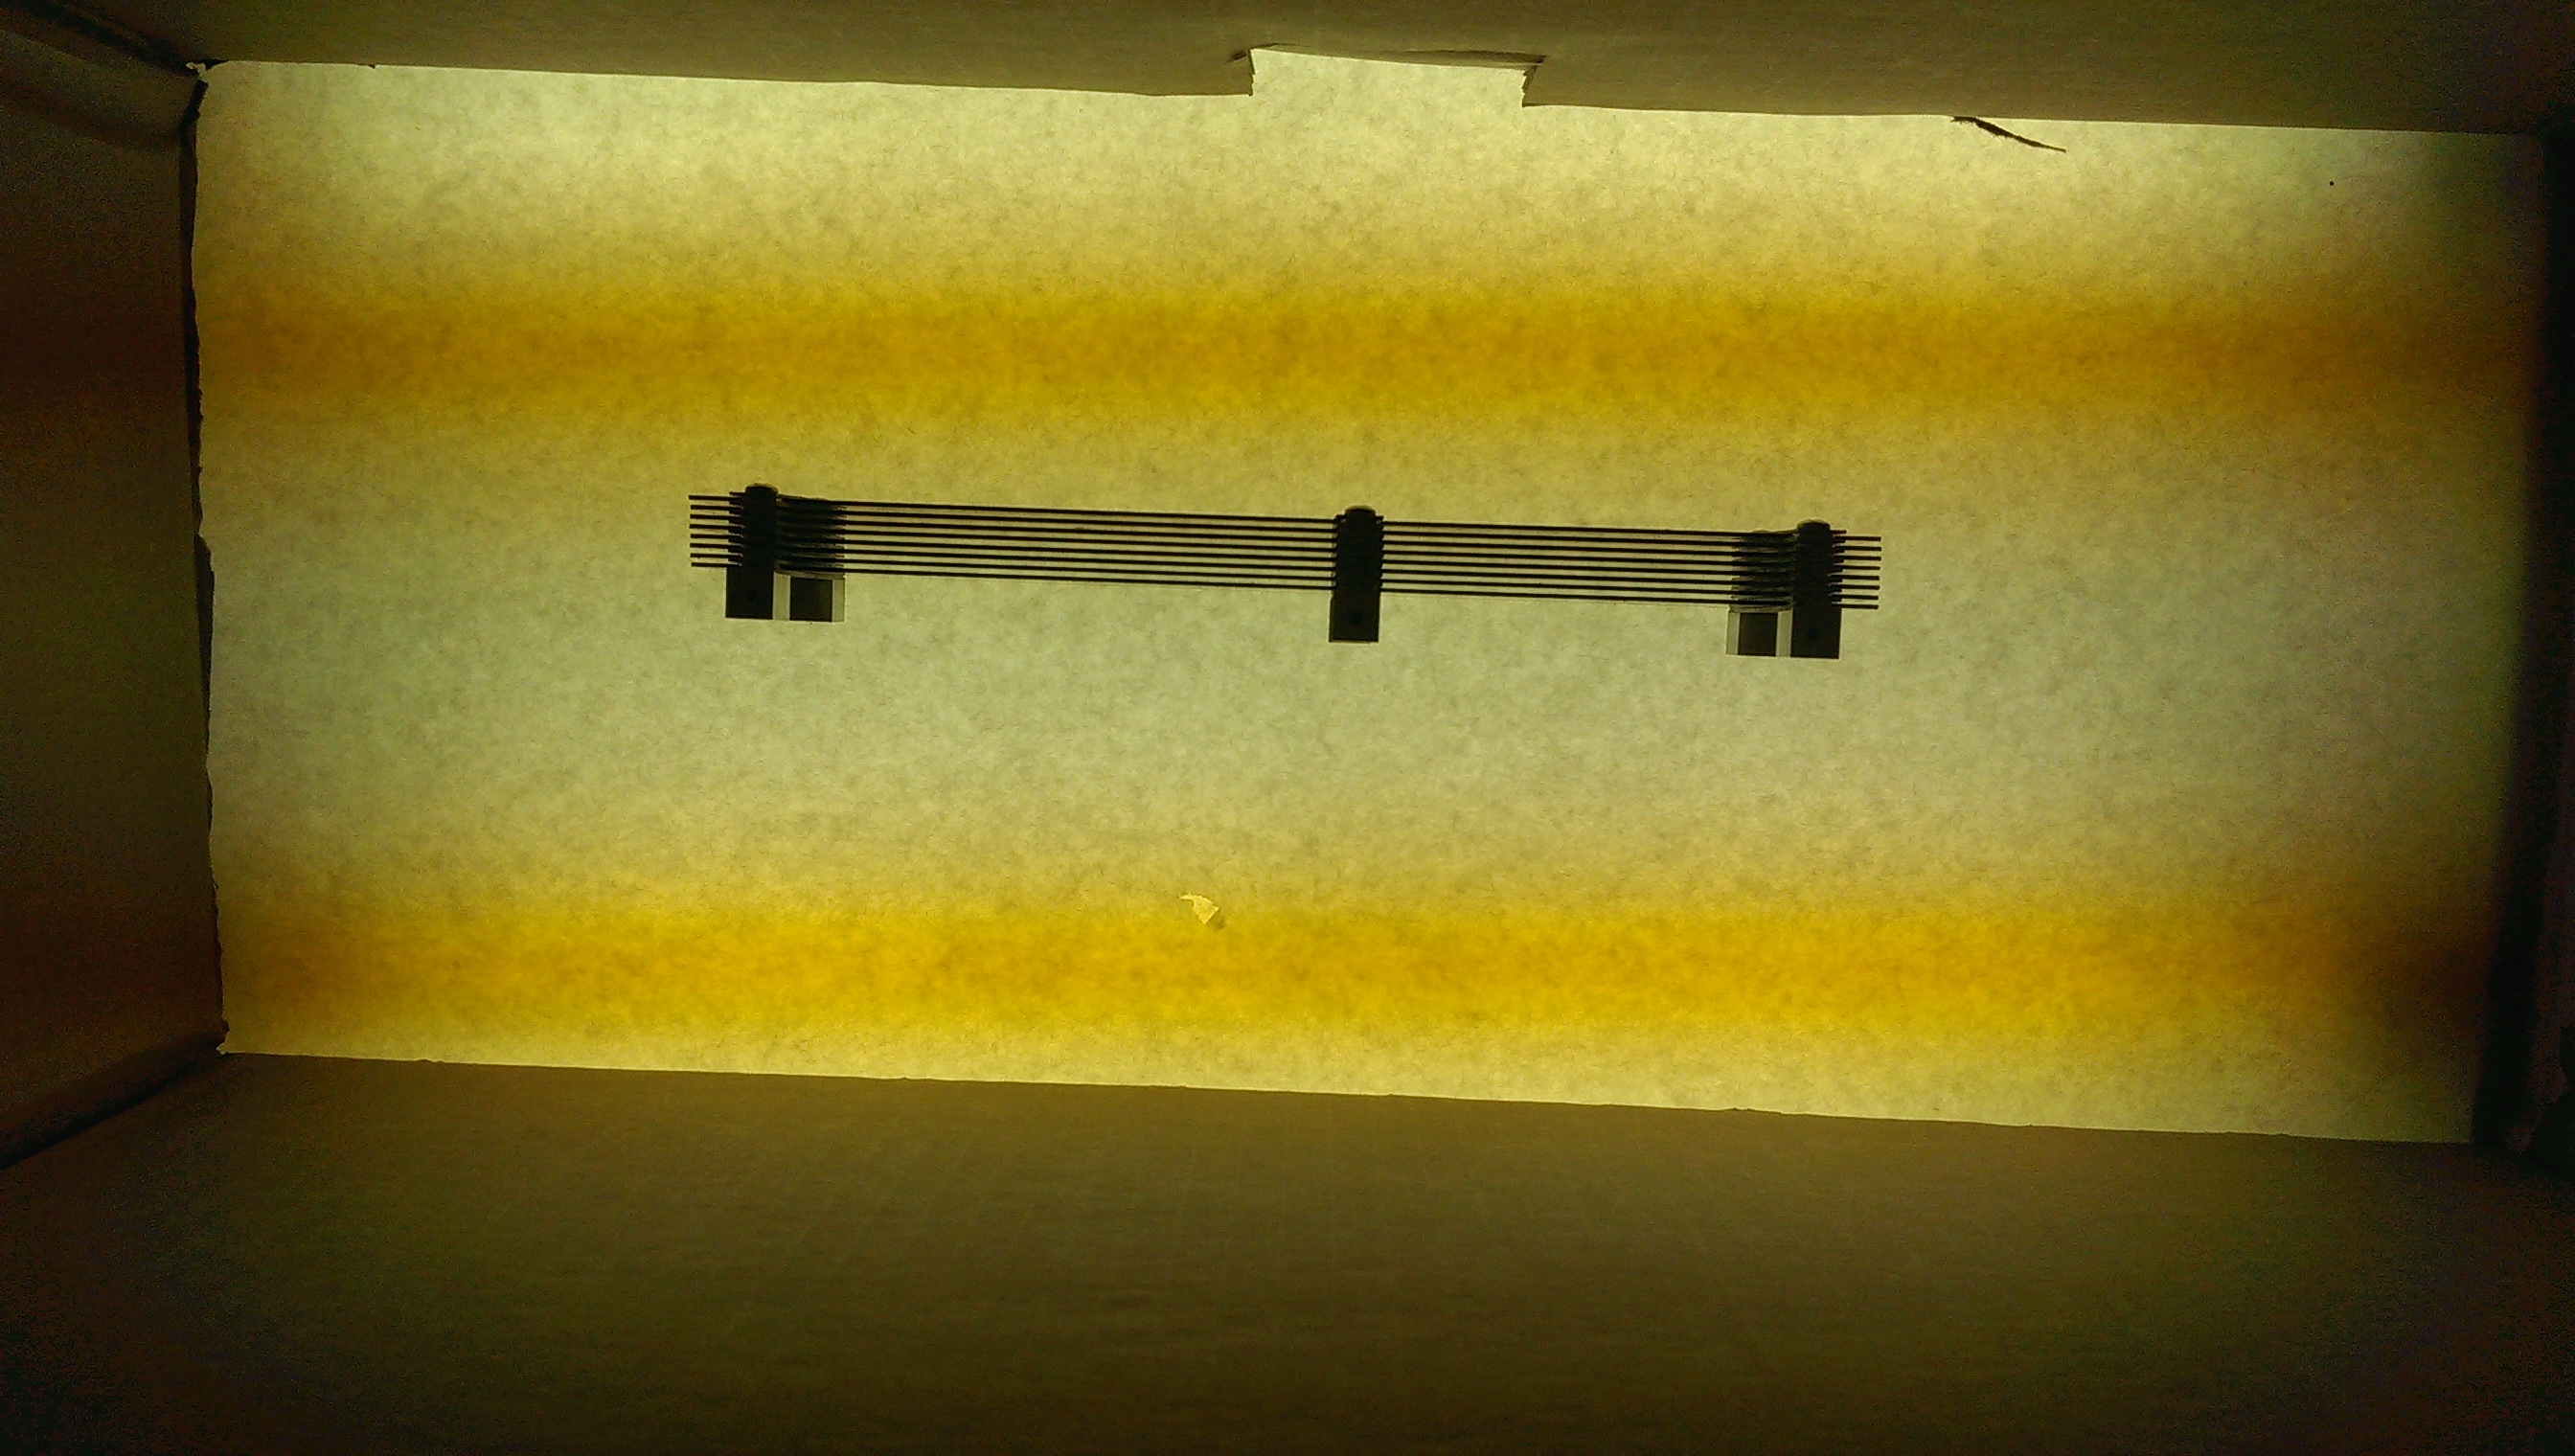
\includegraphics[width=1.3\textwidth]{../plots_tables_images/slats/IMAG0124_BURST002_COVER.jpg}
%         \caption{}
%     \end{subfigure}
%     \hspace{.5in}
%     \begin{subfigure}[b]{.45\linewidth}
%         \centering
%         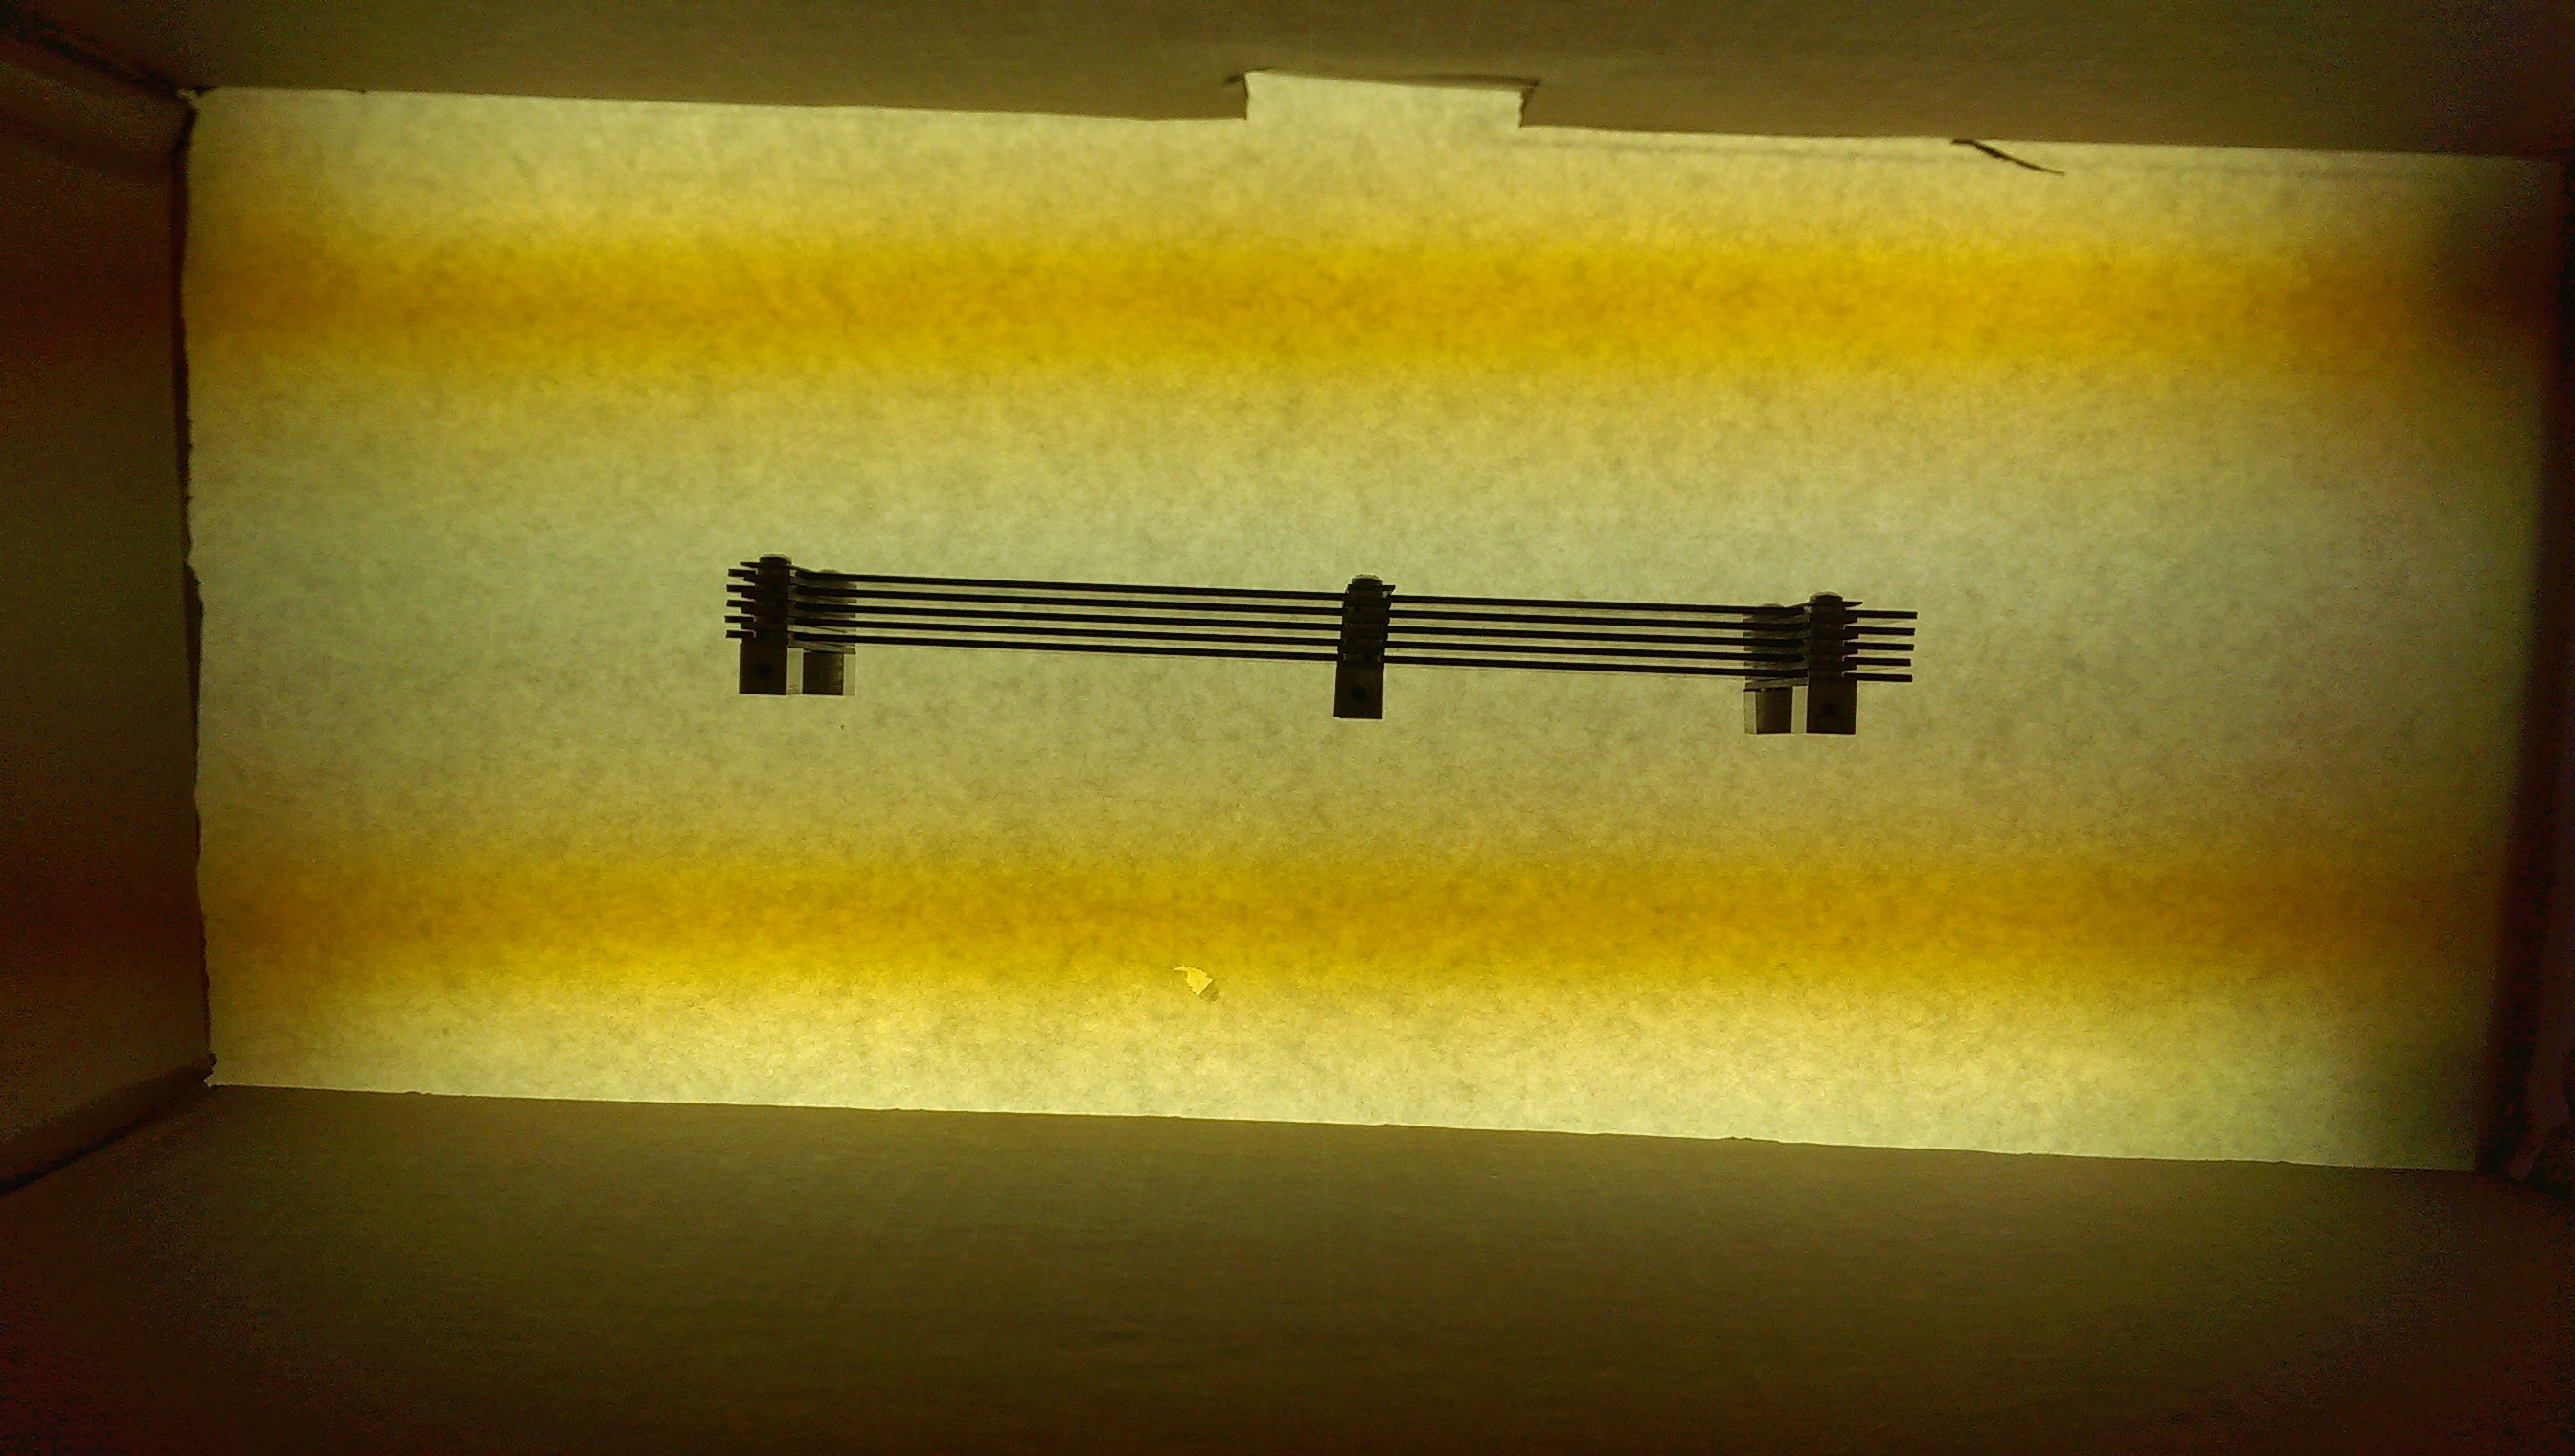
\includegraphics[width=1.3\textwidth]{../plots_tables_images/slats/IMAG0133_BURST003.jpg}
%         \caption{}
%     \end{subfigure}
%     \caption{Even though the images are small you can still zoom in a lot.}
% \end{figure}

Some full-size photos:

\begin{figure}[!ht]
    \centering
    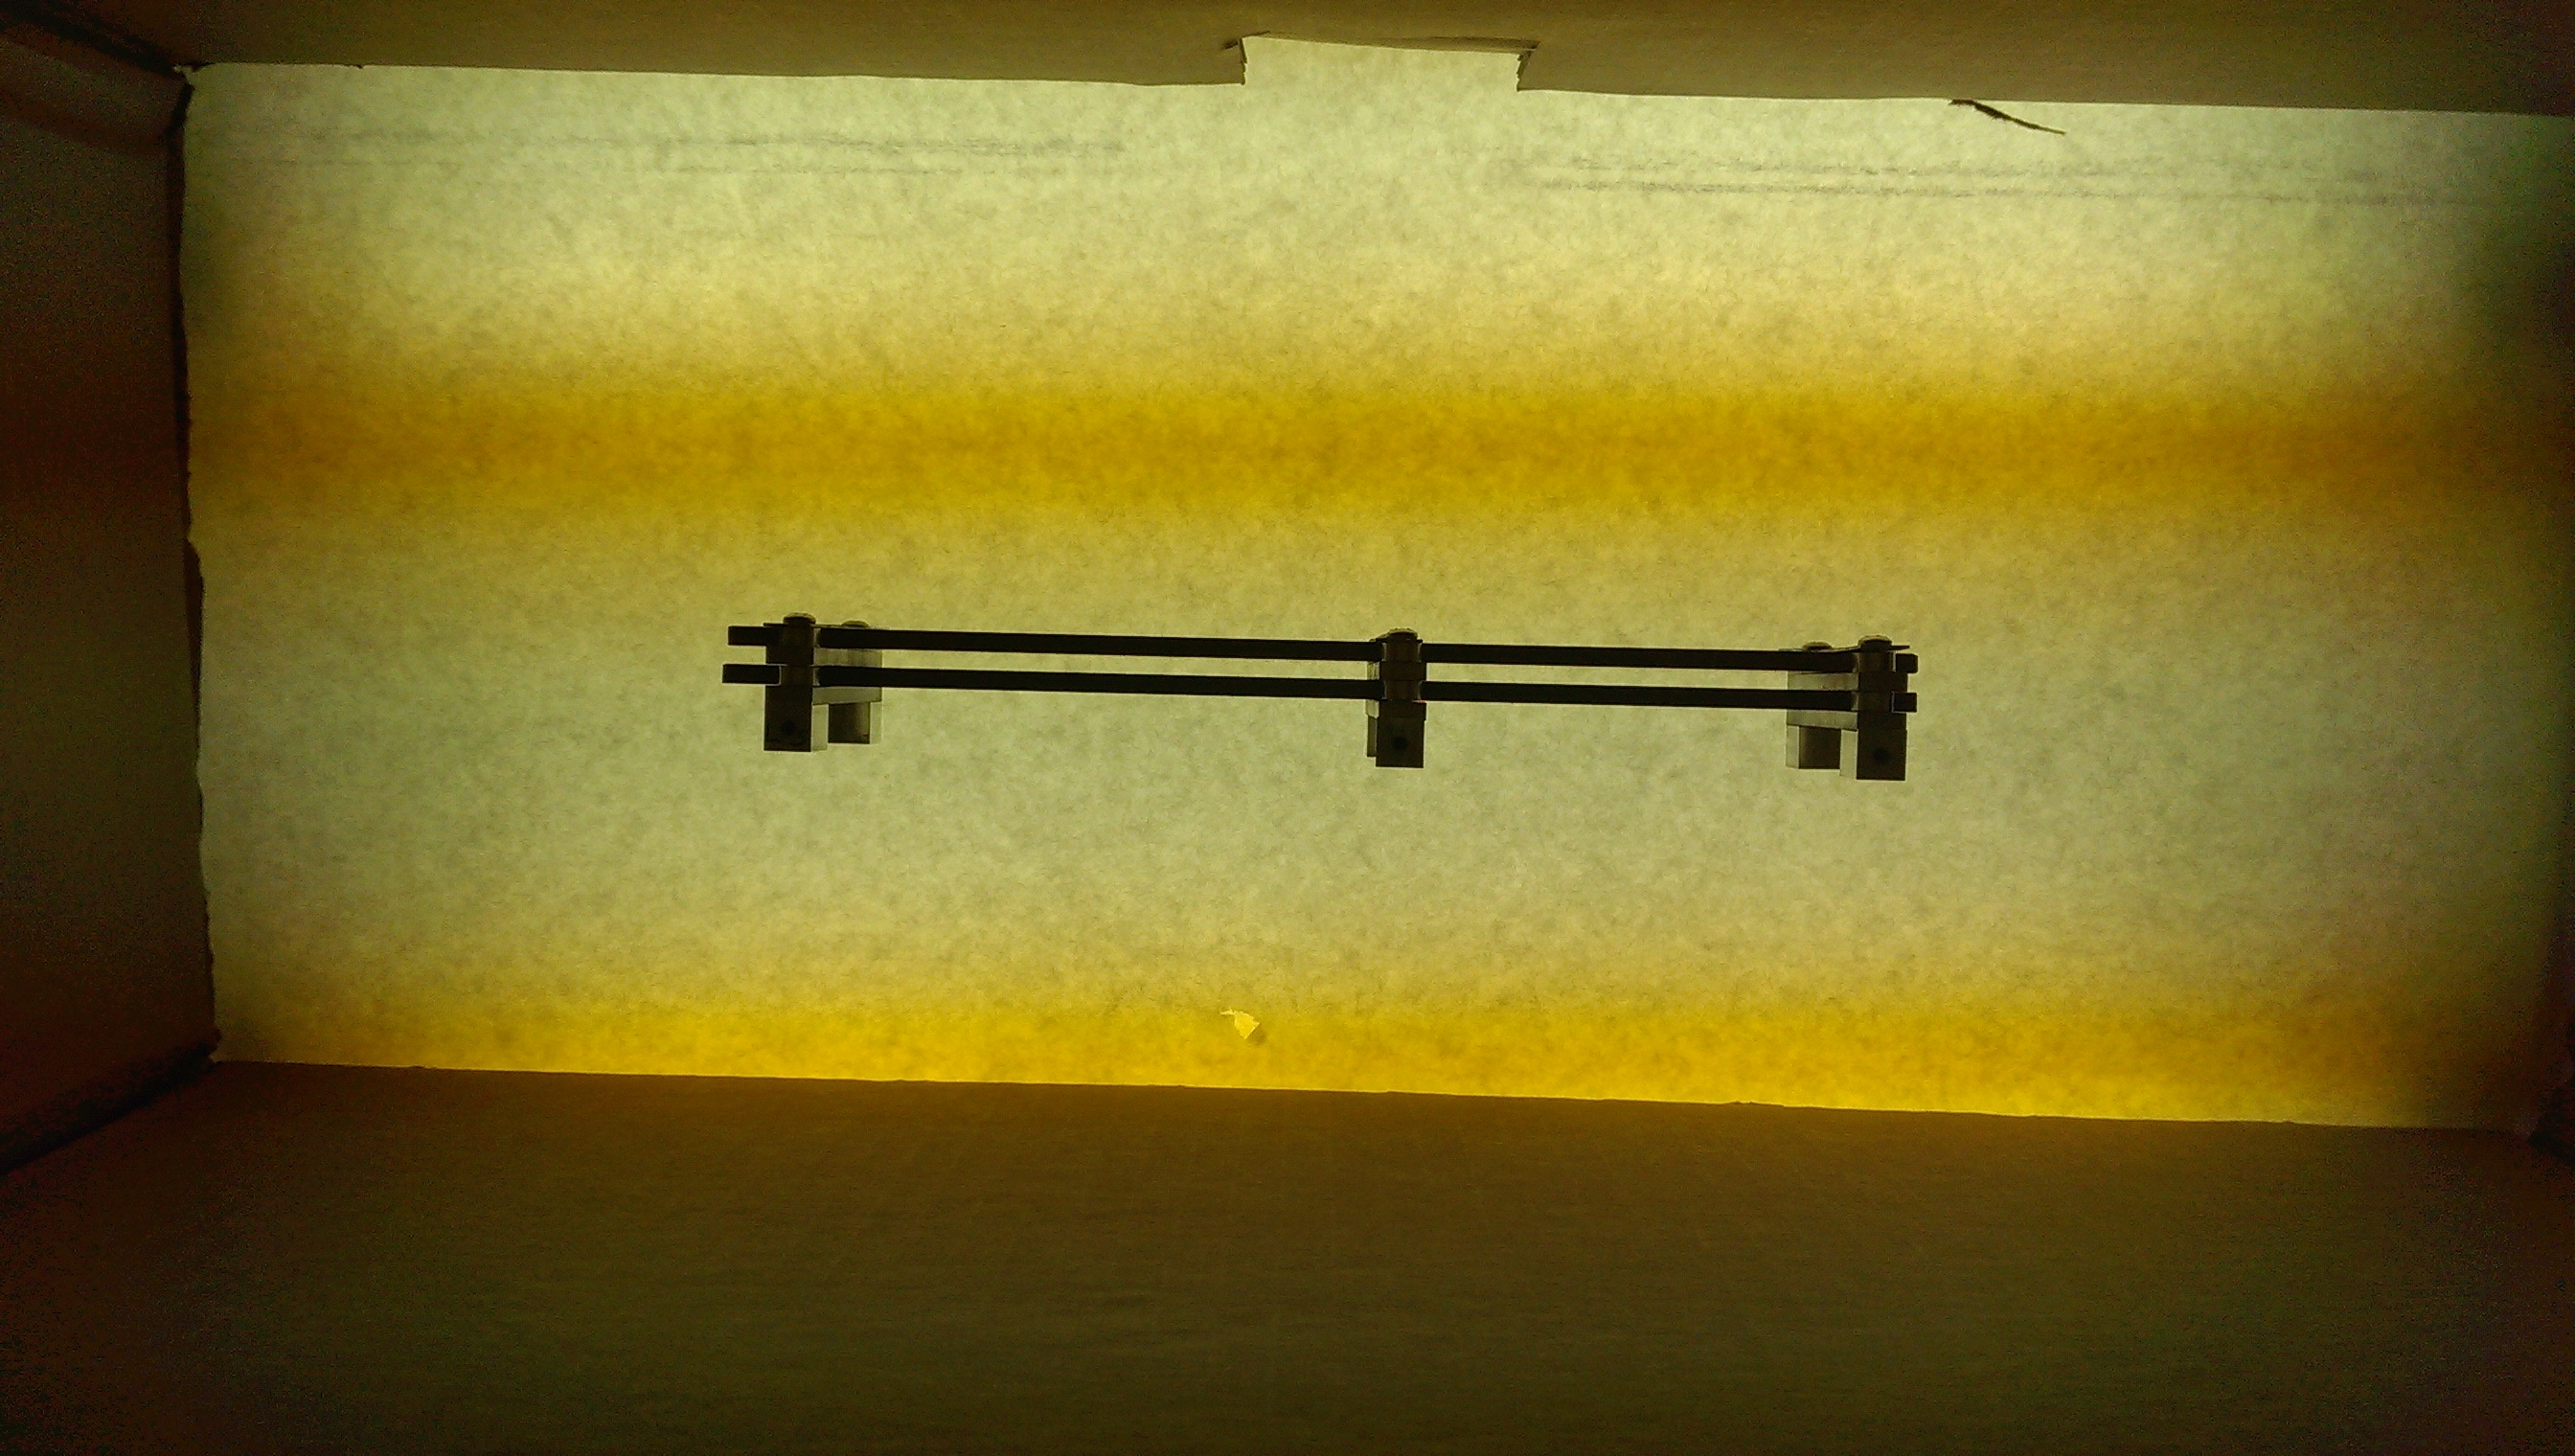
\includegraphics[width=\textwidth]{../plots_tables_images/slats/IMAG0137_BURST010.jpg}
    \caption{}
\end{figure}
\begin{figure}[!ht]
    \centering
    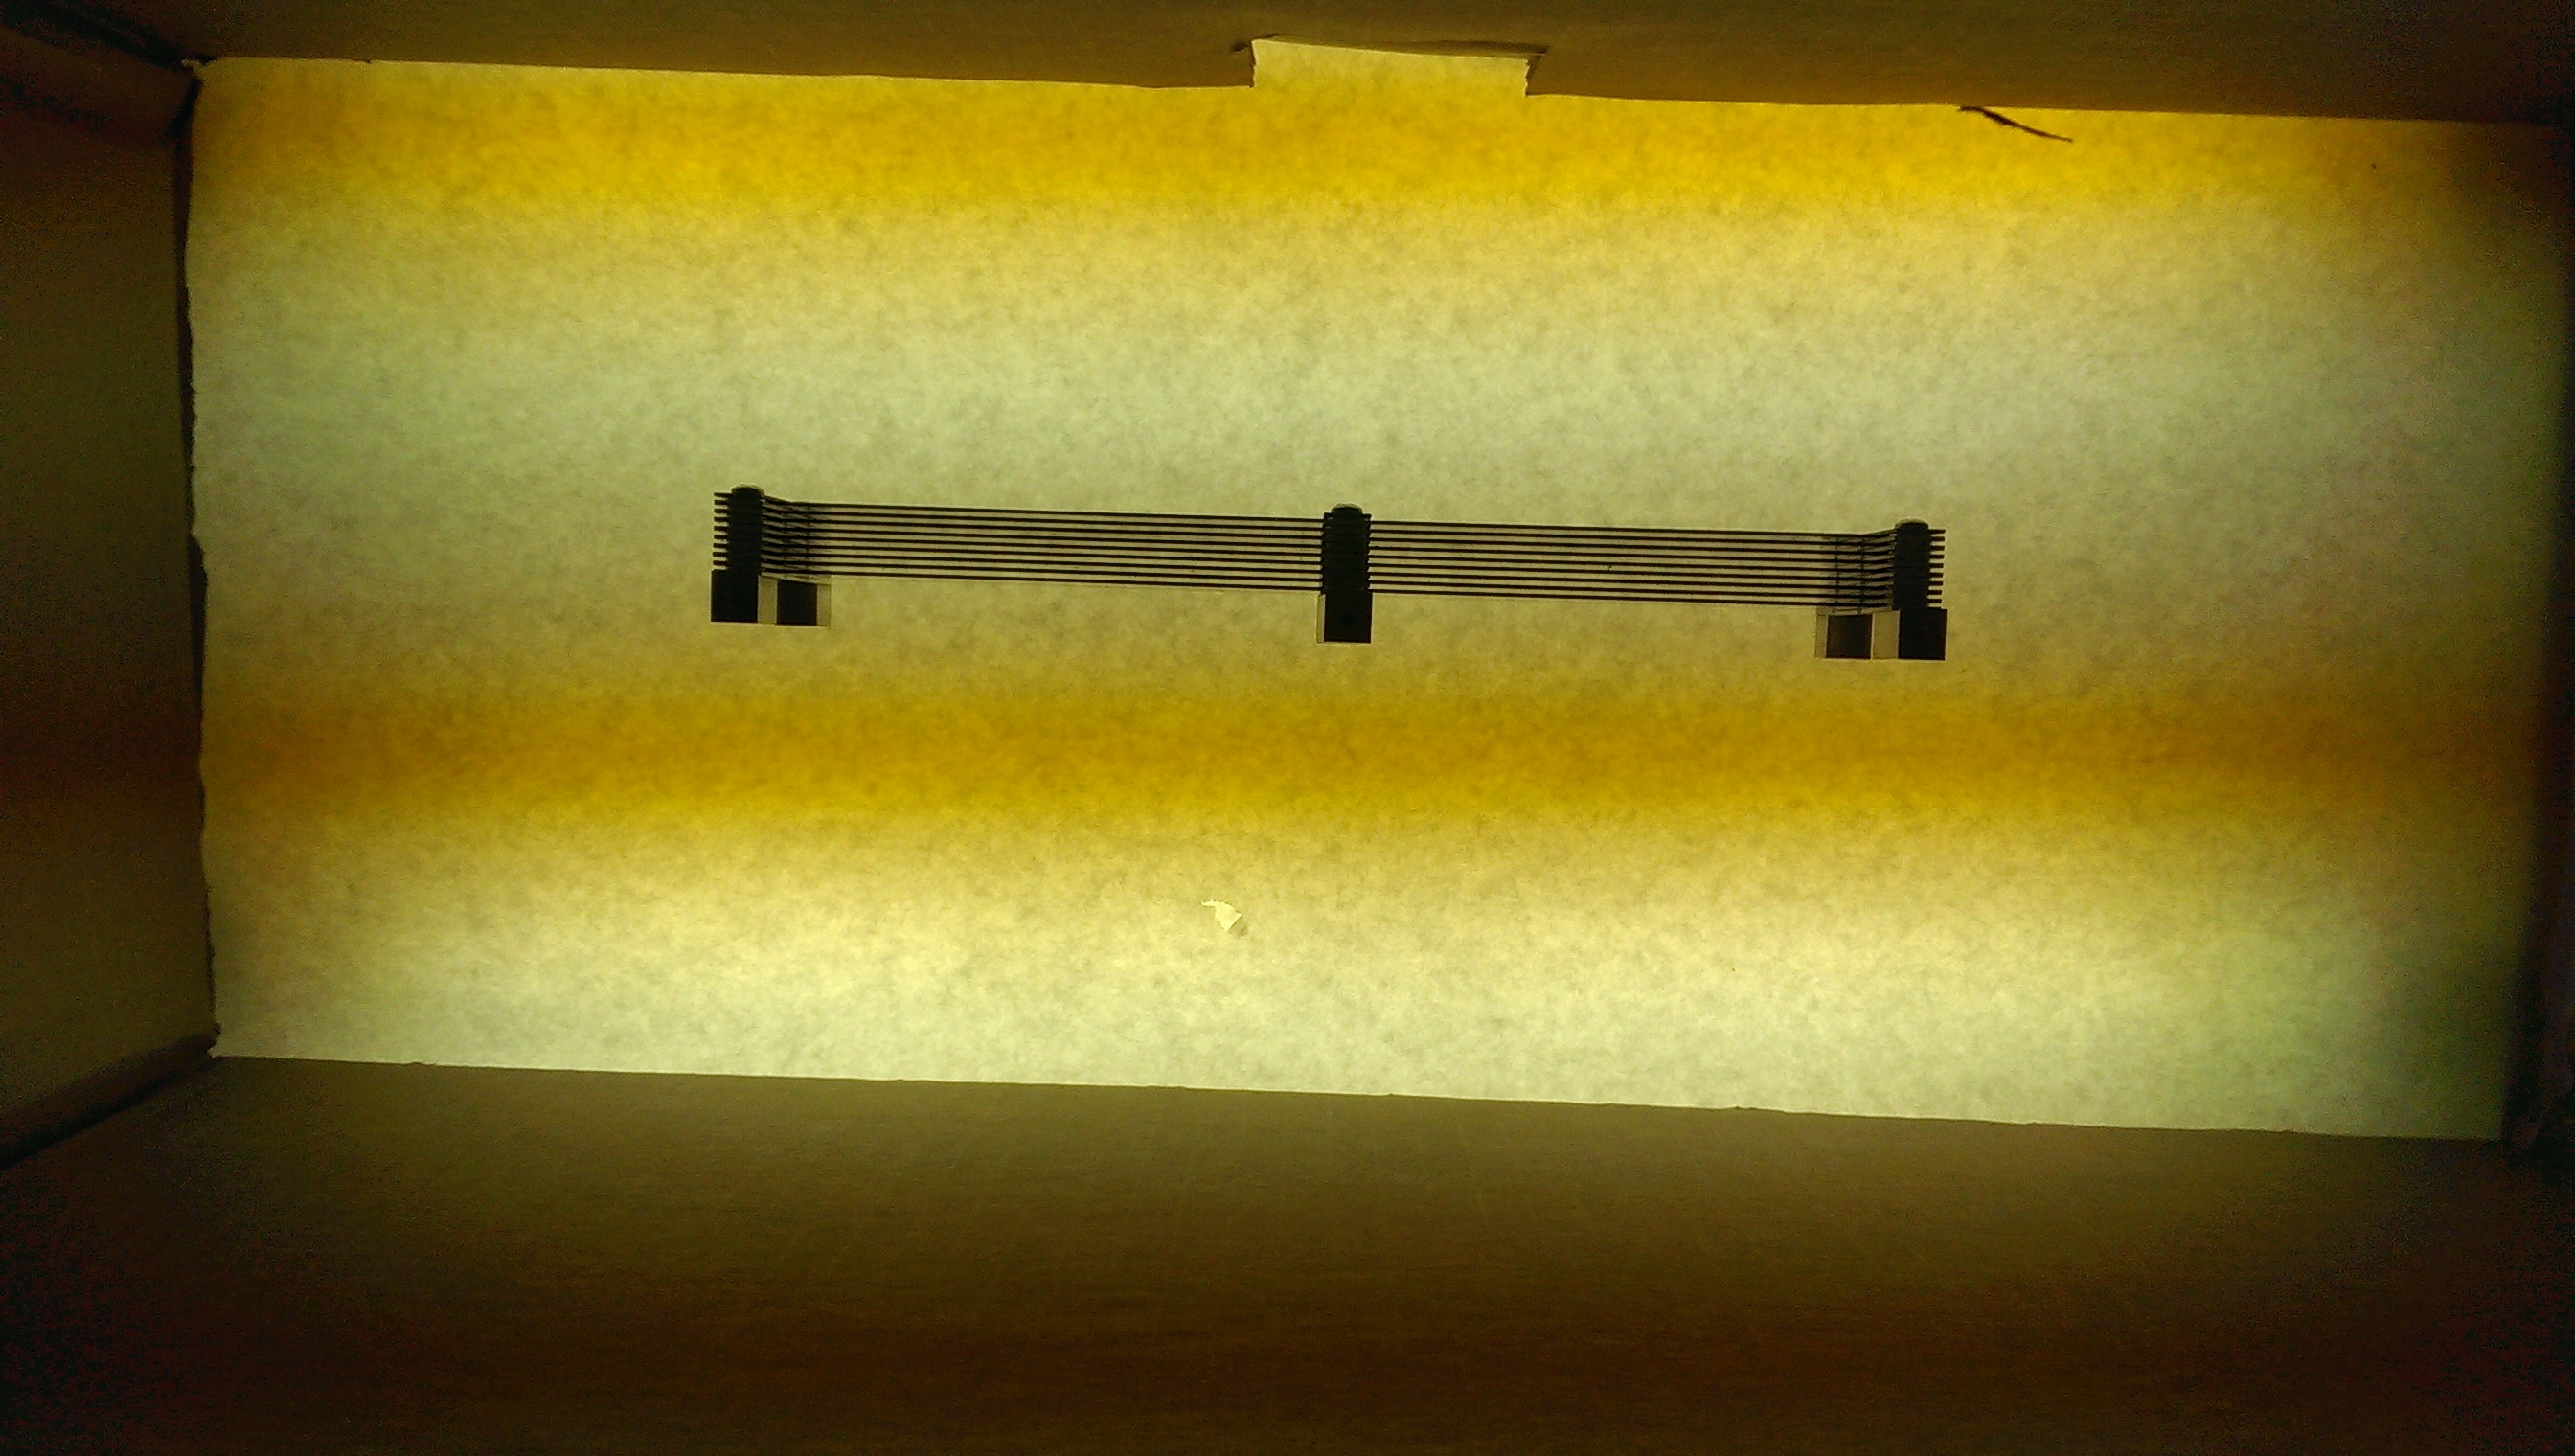
\includegraphics[width=\textwidth]{../plots_tables_images/slats/IMAG0122.jpg}    
    \caption{}
\end{figure}
\begin{figure}[!ht]
    \centering
    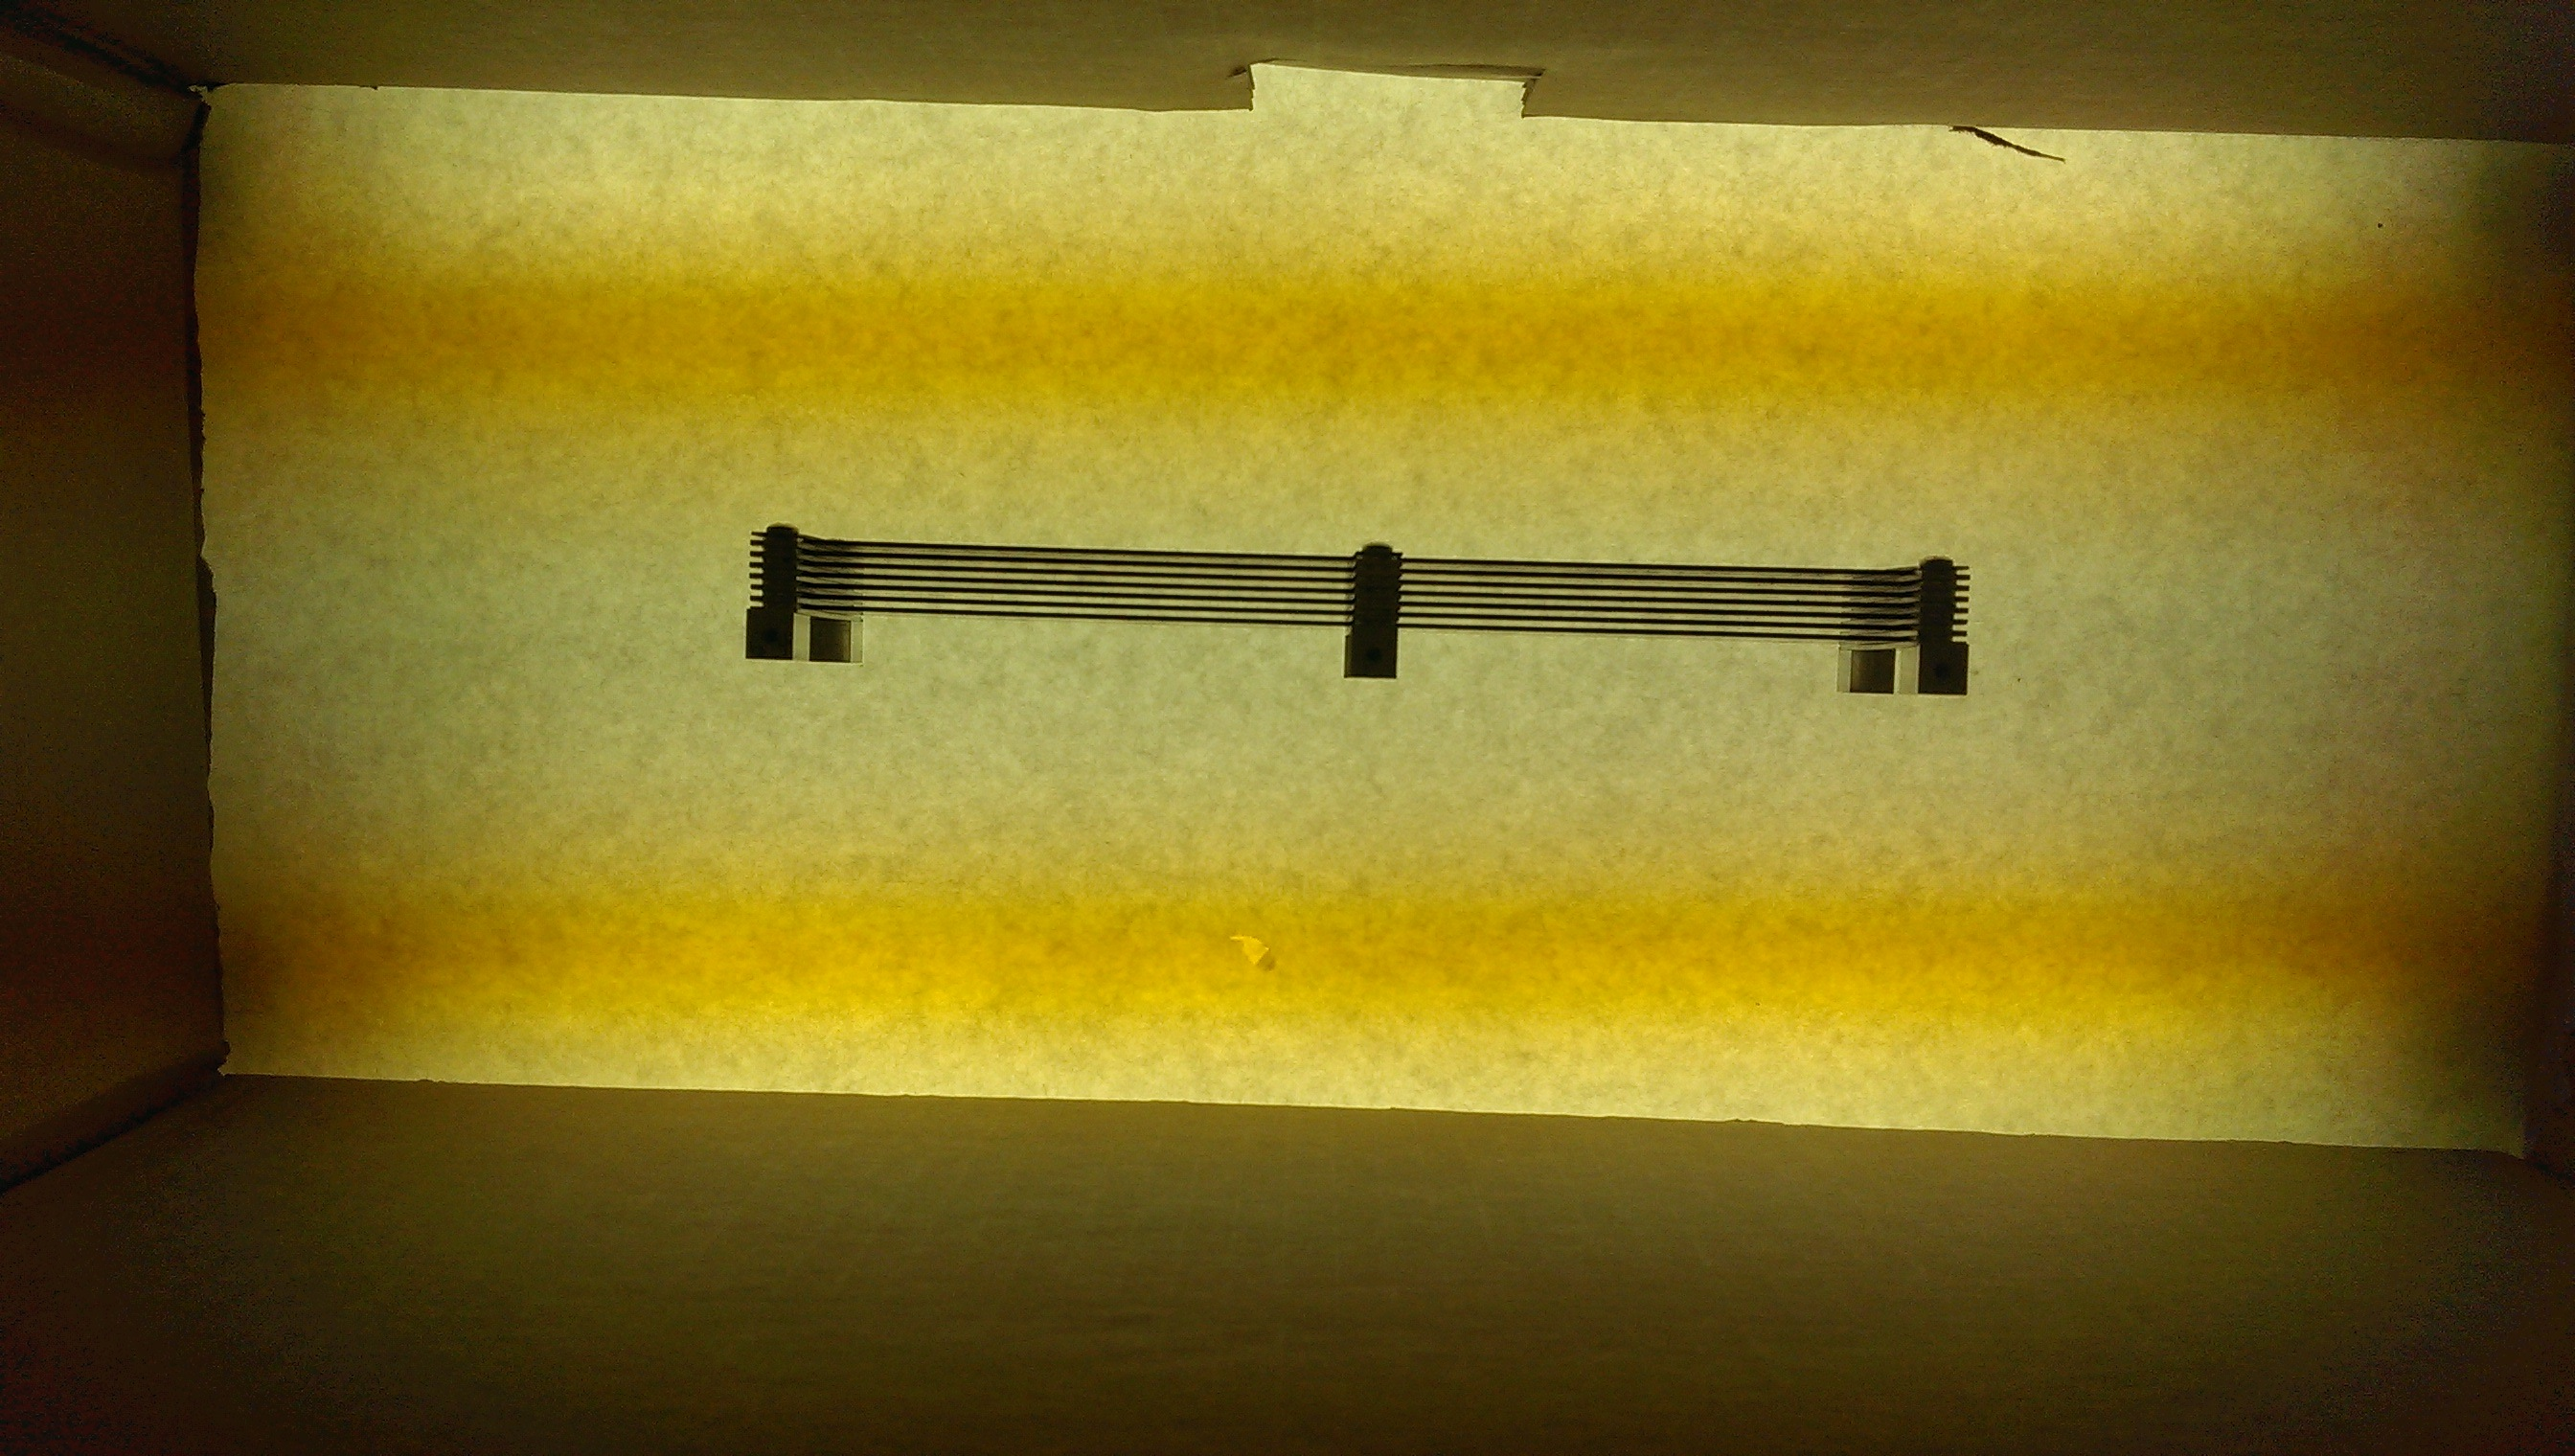
\includegraphics[width=\textwidth]{../plots_tables_images/slats/IMAG0128.jpg}
    \caption{}
\end{figure}

% section with_diffuse_paper (end)

\clearpage
\section{Back light, No diffuse paper} % (fold)
\label{sec:no_diffuse_paper}
This image was taken after the previous set; probably going to use this setup from now on.

\begin{figure}[!ht]
    \centering
    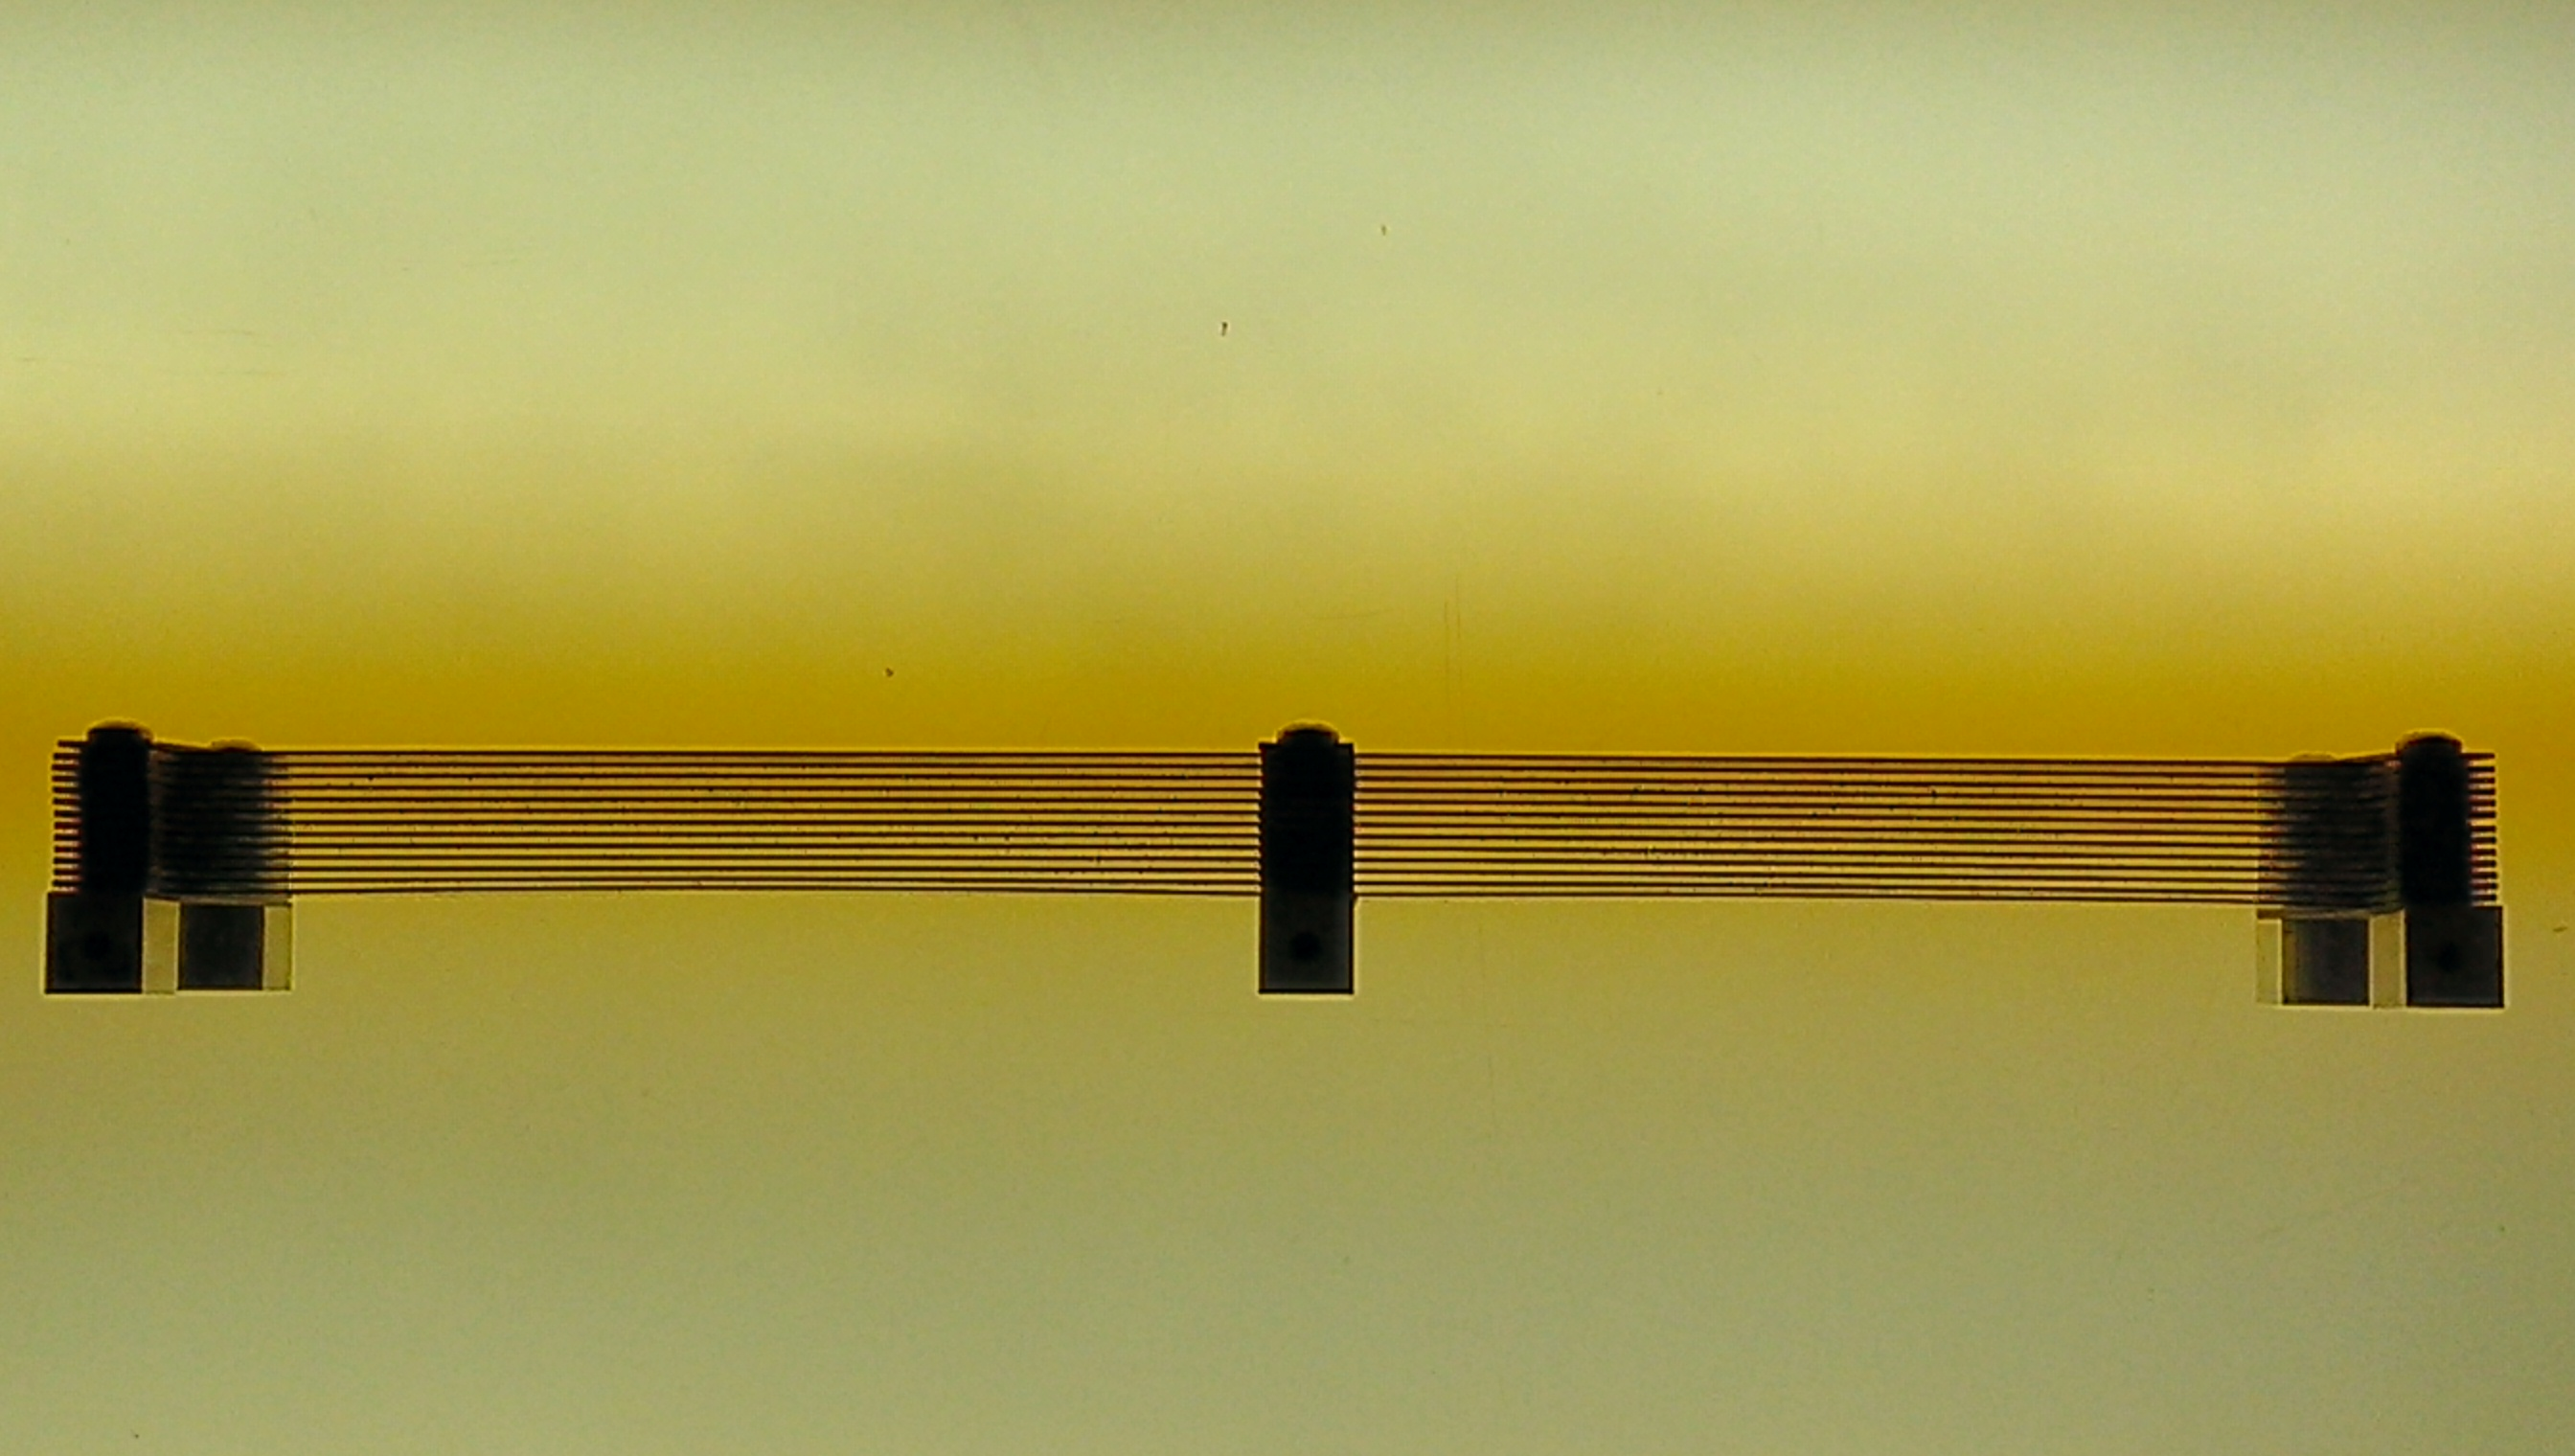
\includegraphics[width=.9\textwidth]{../plots_tables_images/slats/IMAG0147.jpg}    
    \caption{Background lighting, no tissue paper. Zoomed in on camera.}
    \label{flowchart}
\end{figure}

% section no_diffuse_paper (end)


\section{Preferred way to take pictures} % (fold)
\label{sec:preferred_way_to_take_pics}
Backlight with a non-cell phone camera looks like the current best option. The rolling shutter of the cell phone camera combined with fluorescent lighting's flickering properties lead to less-than-ideal photos.
% section preferred_way_to_take_pics (end)


\end{document}